\documentclass[10pt]{article}
\usepackage[a4paper,margin=1in]{geometry}
\usepackage[T1]{fontenc}
\usepackage[utf8]{inputenc}
\usepackage{lmodern}
\usepackage{amsmath,amssymb,amsthm,mathtools}
\usepackage{aliascnt}
\usepackage{microtype}
\usepackage[skip=0.45\baselineskip plus 2pt,indent=0pt]{parskip}
\usepackage{booktabs,array,graphicx}
\usepackage{enumitem}
\usepackage{tikz}
\usetikzlibrary{arrows.meta,positioning}
\usepackage[colorlinks=true,linkcolor=blue,citecolor=blue,urlcolor=blue]{hyperref}
\usepackage[nameinlink,noabbrev]{cleveref}
\hypersetup{pdftitle={Simplified proofs of sharp tail bounds and the Erd\H{o}s matching theorem for large matchings},pdfauthor={}}
\numberwithin{equation}{section}
\newtheorem{theorem}{Theorem}[section]
\newaliascnt{lemma}{theorem}
\newtheorem{lemma}[lemma]{Lemma}
\aliascntresetthe{lemma}
\newaliascnt{proposition}{theorem}
\newtheorem{proposition}[proposition]{Proposition}
\aliascntresetthe{proposition}
\newaliascnt{corollary}{theorem}
\newtheorem{corollary}[corollary]{Corollary}
\aliascntresetthe{corollary}
\newaliascnt{claim}{theorem}
\newtheorem{claim}[claim]{Claim}
\aliascntresetthe{claim}
\theoremstyle{definition}
\newaliascnt{definition}{theorem}
\newtheorem{definition}[definition]{Definition}
\aliascntresetthe{definition}
\newaliascnt{remark}{theorem}
\newtheorem{remark}[remark]{Remark}
\aliascntresetthe{remark}
\crefname{theorem}{theorem}{theorems}
\Crefname{theorem}{Theorem}{Theorems}
\crefname{lemma}{lemma}{lemmas}
\Crefname{lemma}{Lemma}{Lemmas}
\crefname{proposition}{proposition}{propositions}
\Crefname{proposition}{Proposition}{Propositions}
\crefname{corollary}{corollary}{corollaries}
\Crefname{corollary}{Corollary}{Corollaries}
\crefname{claim}{claim}{claims}
\Crefname{claim}{Claim}{Claims}
\crefname{definition}{definition}{definitions}
\Crefname{definition}{Definition}{Definitions}
\crefname{remark}{remark}{remarks}
\Crefname{remark}{Remark}{Remarks}
\DeclareMathOperator{\Var}{Var}
\DeclareMathOperator{\Cov}{Cov}
\DeclareMathOperator{\supp}{supp}
\DeclareMathOperator*{\esssup}{ess\,sup}
\newcommand{\E}{\mathbb E}
\newcommand{\R}{\mathbb R}
\newcommand{\N}{\mathbb N}
\newcommand{\1}{\mathbf 1}
\newcommand{\eps}{\varepsilon}
\setlist[enumerate]{leftmargin=*,itemsep=2pt,topsep=3pt}
\setlist[itemize]{leftmargin=*,itemsep=2pt,topsep=3pt}
\setlength{\emergencystretch}{2em}
\title{\Large\bfseries Simplified proofs of sharp tail bounds and the Erd\H{o}s matching theorem for large matchings}
\author{}
\date{November 20, 2026}
\begin{document}
\maketitle
\begin{abstract}
This paper presents simplified proofs of the breakthrough results of Chi, Sun, and Wang on sharp tail bounds for sums of i.i.d. nonnegative random variables and the Erd\H{o}s matching conjecture for large matchings. All proofs presented here were generated by GPT from their original arguments, with simplifications and expanded details.
\end{abstract}
\section{Introduction}\label{sec:introduction}

Given an integer $k\ge2$, a \emph{$k$-uniform hypergraph}, or \emph{$k$-graph}, is a collection of $k$-subsets of a vertex set. We identify a hypergraph with its edge set and write $|H|$ for its number of edges. A \emph{matching} is a collection of pairwise disjoint edges, and the \emph{matching number} $\nu(H)$ is the largest size of a matching in $H$.

The Erd\H{o}s matching conjecture~\cite[equation (9)]{Erdos1965} asks for the largest number of edges in an $n$-vertex $k$-graph with matching number at most $s$. Two constructions give the proposed answer. For $S\subseteq V$ with $|S|=s$, the \emph{complete $s$-cover} is
\begin{align*}
\mathcal A(V,S)\coloneqq\{E\in\tbinom Vk\colon E\cap S\ne\varnothing\}.
\end{align*}
Each matching in this hypergraph uses a distinct vertex of $S$ for each of its edges. Thus its matching number is at most $s$, and it has $\binom nk-\binom{n-s}k$ edges. The second construction consists of all $k$-sets in a set $Q$ of size $k(s+1)-1$. A matching of size $s+1$ would require one more vertex than $Q$ contains. For later use, set
\begin{align}
M(n,s)&\coloneqq\binom nk-\binom{n-s}k, &
C(s)&\coloneqq\binom{ks+k-1}k, &
D(n,s)&\coloneqq\max\{M(n,s),C(s)\}.
\label{eq:matching-counts}
\end{align}

For $k=4$ and sufficiently large $s$, the conjecture was proved by Hou, Hu, and Liu~\cite{HHL2026}. Chi, Sun, and Wang~\cite[Theorem 1.4]{CSW2026} proved the conjectured bound for every fixed $k$ and all sufficiently large $s$, uniformly over the nontrivial range of $n$.
\begin{theorem}[Chi--Sun--Wang]\label{thm:matching}
For every integer $k\ge3$, there exists $s_0(k)$ such that the following holds. If $s\ge s_0(k)$, $n\ge k(s+1)$, and $H$ is an $n$-vertex $k$-graph with $\nu(H)\le s$, then $|H|\le D(n,s)$. Equality holds only when $H$ is a complete $s$-cover or a complete $k$-graph on $ks+k-1$ vertices, together with isolated vertices. A standard construction is extremal precisely when its size equals $D(n,s)$.
\end{theorem}

The probability theorem behind this result also has two natural extremal constructions. For a probability law $P$ on $[0,\infty)$, let
\begin{align}
m(P)&\coloneqq\int t\,dP(t), &
F_j(P)&\coloneqq\Pr(X_1+\cdots+X_j\ge1),
\label{eq:tail-definition}
\end{align}
where $X_1,\ldots,X_j$ are independent with common law $P$. We put $F_0(P)=0$. For $0\le x\le1/k$, define
\begin{align}
B_x&\coloneqq(1-x)\delta_0+x\delta_1, &
C_{k,x}&\coloneqq(1-kx)\delta_0+kx\delta_{1/k}.
\label{eq:standard-laws}
\end{align}
Both laws have mean $x$. Under $B_x$, the sum reaches one as soon as one sample is nonzero. Under $C_{k,x}$, all $k$ samples must be nonzero. Consequently, $F_k(B_x)=1-(1-x)^k$ and $F_k(C_{k,x})=(kx)^k$.

{\L}uczak, Mieczkowska, and {\v S}ileikis~\cite{LMS2017} conjectured that the larger of these two values is optimal. They proved the bound for $k=3$ and for $k\ge5$ when $x<1/(2k-1)$. The following theorem of Chi, Sun, and Wang~\cite[Theorem 1.2]{CSW2026} gives the bound for all $k$, together with all maximizing laws.
\begin{theorem}[Chi--Sun--Wang]\label{thm:tail}
For every integer $k\ge1$ and every $x\ge0$,
\begin{align}
\sup_{m(P)\le x}F_k(P)=
\begin{cases}
\max\{1-(1-x)^k,(kx)^k\},&0\le x\le1/k,\\
1,&x\ge1/k.
\end{cases}
\label{eq:sharp-tail}
\end{align}
For $k\ge2$, there is a unique $\beta_k\in(0,1/k)$ such that $1-(1-\beta_k)^k=(k\beta_k)^k$. For $0<x<\beta_k$, the unique maximizing law is $B_x$; for $\beta_k<x\le1/k$, it is $C_{k,x}$; at $x=\beta_k$, these are the only two maximizing laws. At $x=0$ the only feasible law is $\delta_0$. For $k=1$ and $0\le x\le1$, the unique maximizing law is $B_x$. For $x>1/k$, a feasible law is maximizing if and only if it is supported on $[1/k,\infty)$.
\end{theorem}

The correspondence between the two theorems comes from vertex weights. The connection between fractional covers and tails of sums of independent samples already appears in Alon, Huang, and Sudakov~\cite[Lemma 3.3]{AHS2012} and Alon, Frankl, Huang, R\"odl, Ruci\'nski, and Sudakov~\cite[proof of Theorem 2.1]{AFHRRS2012}; {\L}uczak, Mieczkowska, and {\v S}ileikis~\cite[Lemma 3.2]{LMS2017} give the corresponding equivalence with the asymptotic fractional matching conjecture. If the vertices in $S$ have weight one and all other vertices have weight zero, a $k$-set has weight at least one exactly when it meets $S$. If the vertices in $Q$ have weight $1/k$, a $k$-set has weight at least one exactly when it lies in $Q$. Writing $x=s/n$, the two edge densities tend to $1-(1-x)^k$ and $(kx)^k$, respectively. The equality classification in \cref{thm:tail} identifies precisely these two configurations in the limit.

We use the approximate fractional-cover statement in Cao, Liu, and Zhang~\cite[Lemma 3.2]{CLZ2026} to apply this correspondence to hypergraphs with bounded matching number. It gives vertex weights of total at most $s+o(n)$ that cover all but $o(n^k)$ edges. An integer matching bound does not give an exact fractional cover of the same weight. For example, the minimum fractional cover weight of the complete $k$-graph on $ks+k-1$ vertices is $(ks+k-1)/k>s$. The role of earlier regularity and rounding arguments is discussed in \cref{sec:stability}.

We present complete proofs of \cref{thm:tail,thm:matching} by simplifying and expanding the arguments of Chi, Sun, and Wang~\cite{CSW2026}. The main theorems are attributed to Chi, Sun, and Wang throughout. The purpose is to make the dependencies, the equality arguments, and the numerical verifications explicit. In particular, no inequality from the technical appendix is left as an unspecified calculation, and the use of approximate covers is separated from the arguments that give exact edge counts. Local citations identify inherited lemmas and distinguish changes in their proofs or quantitative forms.

\paragraph{The probability proof.}
Two mixtures reduce the problem to the mean $x=\beta_k$: adding mass at one treats smaller means, and adding mass at zero treats larger means. A maximizing law has the form $P=(1-kx)\delta_0+kxQ$, where $Q$ is supported on $[0,1]$ and has mean $1/k$. For independent $Y_i\sim Q$, the quantity $w=k\E(Y_1+\cdots+Y_k-1)_+$ lies between zero and $k(1-1/k)^k$. The two endpoints correspond exactly to the two laws in \cref{eq:standard-laws}.

To exclude an interior value of $w$, we first compare the tails and expected excesses of all partial sums. A product lower bound for the failure probability yields concave upper bounds for the partial-sum tails. An interpolation argument combines these bounds with the elementary recurrence between successive excesses. For $k\le5$, this already excludes every interior value of $w$. For larger $k$, it excludes an initial interval and supplies the stronger estimates needed in the remaining range.

The remaining argument uses optimality of the law. The function $z\mapsto\Pr(X_1+\cdots+X_{k-1}\ge1-z)$ lies below an affine function and agrees with it almost everywhere under the maximizing law. This relation determines the conditional law of a sample given failure. A covariance identity then bounds the conditional variance. The bound forces the support into a low interval and a separated high interval. If the low interval has positive conditional mean, a cubic test function produces a contradictory lower bound for the same conditional variance. If its mean is zero, the law is $B_x$. Together with the zero-excess case, this proves the critical-mean classification.

\paragraph{The matching proof.}
The approximate cover theorem and compactness turn \cref{thm:tail} into a stability statement: a hypergraph whose size is close to $D(n,s)$ is close to a standard cover or a standard clique. Near a cover, vertices with almost complete links allow a greedy extension of any residual matching; the resulting smaller matching problem has an elementary exact solution. Near a clique, shifting first reveals a genuine large clique. We then count edges according to the number of vertices outside it. Random disjoint blocks in the clique give a bipartite graph, and K\H{o}nig's theorem bounds the edges with exactly one outside vertex. A deficit in this bound controls all possible gains from edges with several outside vertices, with a coefficient strictly smaller than one. This gives the exact clique bound and its equality case.

\paragraph{Organization and notation.}
\Cref{sec:reduction} gives the normalization and critical-mean reduction. \Cref{sec:comparison} develops the product and interpolation arguments. \Cref{sec:support,sec:exclusion} prove the support restriction and exclude the remaining maximizing laws, and \cref{sec:equality} completes \cref{thm:tail}. \Cref{sec:stability,sec:exact} prove stability and the exact matching theorem. The appendix proves the numerical estimates used in the probability argument. We write $[j]=\{1,\ldots,j\}$, $u_+=\max\{u,0\}$, and $A\triangle B$ for symmetric difference. All random variables declared as copies of a law are independent unless a conditioning is explicitly stated. The integer $t$ indexes comparison nodes in the probability proof; the letter $s$ is reserved for the matching parameter in the hypergraph sections.

\section{Reduction to the critical mean}\label{sec:reduction}

Fix an integer $k\ge2$. We follow the critical-mean reduction of Chi, Sun, and Wang~\cite[Section 2.1]{CSW2026}. We first identify the mean at which the two proposed extremal distributions give the same probability. We then show that a proof at this mean determines both the optimal value and the maximizing distributions at every other mean.

For $c\ge0$, define
\begin{align*}
 g_k(c)\coloneqq \left(1+\frac ck\right)^k-\left(1+\frac{c-1}{k}\right)^k.
\end{align*}
Its derivative is positive, $g_k(0)<1$, and $g_k(1)>1$. Thus there is a unique $c_k\in(0,1)$ such that $g_k(c_k)=1$. Define
\begin{align}\label{eq:critical-parameters}
 \beta_k\coloneqq\frac1{k+c_k}.
\end{align}
For $x\in(0,1/k)$, substituting $c=1/x-k$ gives
\begin{align*}
 1-(1-x)^k-(kx)^k=(kx)^k\bigl(g_k(c)-1\bigr).
\end{align*}
Consequently, $\beta_k$ is the unique crossing point of the two proposed bounds in $(0,1/k)$; the Bernoulli expression is larger for $x<\beta_k$, and the other expression is larger for $x>\beta_k$.

For example, when $k=3$, the crossing equation reduces to $26\beta_3^2+3\beta_3-3=0$, so $\beta_3=(\sqrt{321}-3)/52$. The two candidate probabilities are shown in \cref{fig:critical-mean}. The reduction below explains why proving the bound at their intersection is sufficient.
\begin{figure}[ht]
\centering
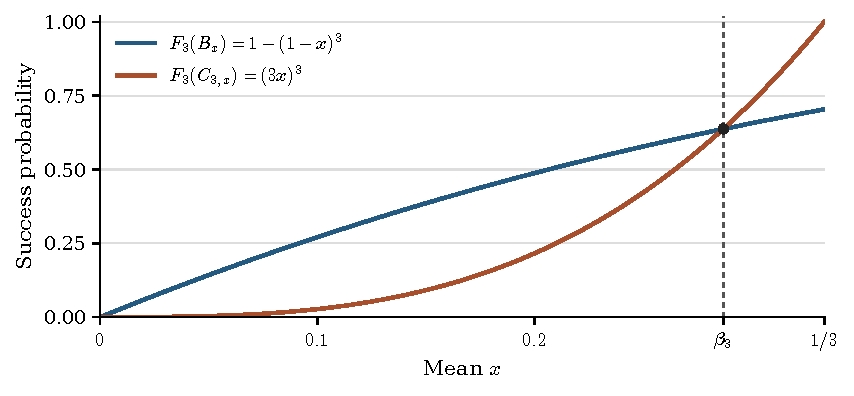
\includegraphics[width=0.76\textwidth]{figures/critical_mean.pdf}
\caption{The two candidate probabilities when $k=3$. Their unique intersection in $(0,1/3)$ occurs at $\beta_3\approx0.286855$. The larger curve gives the sharp bound.}
\label{fig:critical-mean}
\end{figure}

We will repeatedly use $c_k\le1/2$, with equality only when $k=2$. To see this, expand $g_k(1/2)$ about $1$:
\begin{align*}
 g_k(1/2)=2\sum_{\substack{h\in[k]\\ h\text{ odd}}}\binom kh(2k)^{-h}.
\end{align*}
The term with $h=1$ is $1$. The remaining terms vanish when $k=2$ and include a positive term when $k\ge3$. The assertion follows from the strict increase of $g_k$.

The following two mixing operations explain why the crossing point is the appropriate mean to study. For any nonnegative law $P$ and $0\le\vartheta,q\le1$, independence gives
\begin{align}
 1-F_k\bigl((1-\vartheta)P+\vartheta\delta_1\bigr)
   &=(1-\vartheta)^k\bigl(1-F_k(P)\bigr),\label{eq:mix-one}\\
 F_k\bigl(qP+(1-q)\delta_0\bigr)
   &=\sum_{j\in[k]}\binom kj q^j(1-q)^{k-j}F_j(P)
     \ge q^kF_k(P).\label{eq:mix-zero}
\end{align}
For the first identity, failure requires that none of the $k$ samples come from the added atom at $1$. For the second, condition on the number of samples drawn from $P$; a sample drawn from the added atom contributes zero.

Suppose for the moment that the proposed upper bound has been proved at mean $\beta_k$. If $m(P)=x<\beta_k$, set $\vartheta=(\beta_k-x)/(1-x)$. The mixed law in \cref{eq:mix-one} has mean $\beta_k$, and $1-\vartheta=(1-\beta_k)/(1-x)$. It follows that
\begin{align*}
 (1-\vartheta)^k\bigl(1-F_k(P)\bigr)\ge(1-\beta_k)^k,
 \qquad F_k(P)\le1-(1-x)^k.
\end{align*}
If $\beta_k<x<1/k$, set $q=\beta_k/x$. Applying the critical-mean bound to \cref{eq:mix-zero} gives $q^kF_k(P)\le(k\beta_k)^k$, and hence $F_k(P)\le(kx)^k$. A law with mean less than $x<1/k$ can first be mixed with $\delta_1$ to raise its mean to $x$. This does not decrease its success probability. The cases $x=0$ and $x\ge1/k$ will be treated together with equality in \cref{sec:equality}.

Before studying the critical mean, we establish existence and a useful description of every maximizing law. These conclusions are given in Chi, Sun, and Wang~\cite[Lemma 2.7 and Proposition 2.10]{CSW2026}. The proof below obtains the normalization by an elementary truncation and rescaling argument. The description supplies the atom at zero that is needed for the variations used later.

\begin{lemma}\label{lem:normalization}
Let $0<x<1/k$. A law maximizing $F_k(P)$ subject to $m(P)\le x$ exists. Every maximizing law is supported on $[0,1]$, has mean $x$, and satisfies $P((0,1])\le kx$. In particular, it has a representation
\begin{align}\label{eq:normalized-law}
 P=(1-kx)\delta_0+kxQ,
 \qquad \supp Q\subseteq[0,1],
 \qquad m(Q)=1/k.
\end{align}
\end{lemma}

\begin{proof}
Replacing a nonnegative random variable $X$ by $\min\{X,1\}$ preserves the event that a sum of $k$ such variables is at least $1$. It also cannot increase the mean. We may therefore first maximize over laws on $[0,1]$. These laws form a compact space in the weak topology, and the mean constraint defines a closed subset. If $P_n$ converges weakly to $P$, then $P_n^{\otimes k}$ converges weakly to $P^{\otimes k}$. Since $\{(y_1,\ldots,y_k)\colon\sum_i y_i\ge1\}$ is closed, the Portmanteau theorem, in the form given by Billingsley~\cite{Billingsley1999}, yields
\begin{align*}
 F_k(P)\ge\limsup_{n\to\infty}F_k(P_n).
\end{align*}
Thus the maximum is attained.

Markov's inequality gives $F_k(P)\le kx<1$ for every feasible law. If a maximizing law had mean less than $x$, mixing it with a sufficiently small positive mass at $1$ would remain feasible and would strictly increase its success probability by \cref{eq:mix-one}. Every maximizing law therefore has mean $x$. This also rules out mass above $1$ in an original, untruncated maximizing law: truncation would preserve its success probability and strictly decrease its mean, after which the same mixing operation would improve it.

It remains to bound the mass outside zero. Let $X$ have a maximizing law, and fix $0<t<1/k$. Consider
\begin{align*}
 T_t(X)\coloneqq\frac{(X-t)_+}{1-kt}.
\end{align*}
For every nonnegative sample $(X_1,\ldots,X_k)$ with sum at least $1$,
\begin{align*}
 \sum_{i\in[k]}(X_i-t)_+\ge\sum_{i\in[k]}X_i-kt\ge1-kt.
\end{align*}
Thus this transformation preserves every successful sample. Its mean must be at least $x$; otherwise its law would be a maximizing feasible law with mean less than $x$, which we have just excluded. Since $\E X=x$, this gives
\begin{align*}
 \frac{x-\E\min\{X,t\}}{1-kt}\ge x,
 \qquad \E\min\{X,t\}\le kxt.
\end{align*}
Divide by $t$ and let $t\downarrow0$. Bounded convergence gives $\Pr(X>0)\le kx$. We may consequently subtract mass $1-kx$ from the atom at zero and divide the remaining measure by $kx$. The resulting probability measure $Q$ satisfies \cref{eq:normalized-law}.
\end{proof}

We will prove the following statement at the critical mean. It includes the equality information that will later identify near-extremal hypergraphs.

\begin{proposition}\label{prop:critical}
For every integer $k\ge2$, the maximum of $F_k(P)$ over nonnegative laws with mean at most $\beta_k$ is
\begin{align*}
 (k\beta_k)^k=1-(1-\beta_k)^k.
\end{align*}
The only maximizing laws are $B_{\beta_k}$ and $C_{k,\beta_k}$.
\end{proposition}

Both displayed laws have the required mean and attain the stated value. By \cref{lem:normalization}, it is therefore enough to show that any maximizing law at mean $\beta_k$ is one of these two laws. The next section places its normalized law $Q$ in a family of probability inequalities. For $k\le5$, these inequalities already give the desired classification. For $k\ge6$, \cref{sec:support,sec:exclusion} use the additional optimality of $P$ to exclude the remaining possibilities. We complete the proof of \cref{prop:critical} and return to general means in \cref{sec:equality}.

\section{Probability bounds and interpolation}\label{sec:comparison}

The normalization in \cref{lem:normalization} fixes the mean of $Q$ at $1/k$. We will compare the probabilities that its partial sums reach $1$ with the expected amounts by which those sums exceed $1$. A bound for independent variables with possibly different distributions supplies these comparisons. We prove that bound first, keeping track of the conditional deficit because it will also be used in \cref{sec:exclusion}.

\subsection{A product bound for the failure probability}

Let $S$ be a sum of independent nonnegative variables. Conditional on $S<1$, the mean of $1-S$ records how far a typical unsuccessful sum lies below the threshold. The next lemma combines the truncation argument and product bound of Chi, Sun, and Wang~\cite[Lemmas 2.11--2.12]{CSW2026} to bound this probability in terms of the conditional deficit and the individual means.

\begin{lemma}\label{lem:product}
Let $j\ge1$, let $X_1,\ldots,X_j$ be independent bounded nonnegative random variables, and define
\begin{align*}
 S\coloneqq\sum_{i\in[j]}X_i,
 \qquad p\coloneqq\Pr(S<1)>0,
 \qquad r\coloneqq\E[1-S\mid S<1],
 \qquad B\coloneqq r-1+\E S.
\end{align*}
If $r>\max_{i\in[j]}\E X_i$, then there exist $z_1,\ldots,z_j$ such that
\begin{align}\label{eq:product-bound}
 p\ge\prod_{i\in[j]}\left(1-\frac{z_i}{r}\right),
 \qquad 0\le z_i\le\E X_i,
 \qquad \sum_{i\in[j]}z_i=B.
\end{align}
\end{lemma}

\begin{proof}
We first assume that each variable has finite support. The proof repeatedly replaces a nonconstant coordinate by a capped version of that coordinate. We choose each cap so that the conditional deficit does not decrease, and record the resulting decrease in $B$.

Suppose that at least one coordinate is nonconstant. Since
\begin{align*}
 \sum_{i\in[j]}\Cov(S,X_i\mid S<1)=\Var(S\mid S<1)\ge0,
\end{align*}
there is a nonconstant coordinate $X_i$ with $\Cov(S,X_i\mid S<1)\ge0$. Constant coordinates contribute zero to this sum, so one may indeed choose a nonconstant coordinate. Write $T=S-X_i$ and $\supp X_i=\{x_1<\cdots<x_N\}$. Define
\begin{align*}
 K(t)&\coloneqq\E\bigl[(1-r-T-t)\1_{\{T+t<1\}}\bigr],\\
 A_q&\coloneqq\E\bigl[K(X_i)\1_{\{X_i\le x_q\}}\bigr]
 \quad (1\le q\le N),
 \qquad A_0\coloneqq0.
\end{align*}
The definition of $r$ gives $A_N=0$. Also,
\begin{align*}
 \E[X_iK(X_i)]
 &=\E\bigl[X_i(1-r-S)\1_{\{S<1\}}\bigr]
 =-p\Cov(S,X_i\mid S<1).
\end{align*}
Applying summation by parts to the left side therefore yields
\begin{align*}
 \sum_{q<N}(x_{q+1}-x_q)A_q
 =p\Cov(S,X_i\mid S<1)\ge0.
\end{align*}
Thus some $q<N$ satisfies $A_q\ge0$. Choose the first such $q$. Since $A_{q-1}\le0$ and $\Pr(X_i=x_q)>0$, the identity
\begin{align*}
 A_q-A_{q-1}=\Pr(X_i=x_q)K(x_q)
\end{align*}
implies $K(x_q)\ge0$.

Replace $X_i$ by $X_i'\coloneqq\min\{X_i,x_q\}$, and use primes for the corresponding parameters. The new sum is no larger than the old sum, so $p'\ge p$. Splitting according to whether $X_i\le x_q$ gives
\begin{align*}
 p'(r'-r)
 =\E\bigl[(1-r-T-X_i')\1_{\{T+X_i'<1\}}\bigr]
 =A_q+\Pr(X_i>x_q)K(x_q)\ge0.
\end{align*}
Hence $r'\ge r$ as required.

We next quantify the change in the failure probability. For an arbitrary cap $\tau$, put $X_i'=\min\{X_i,\tau\}$ and $d\coloneqq\E(X_i-\tau)_+$. The pointwise inequality
\begin{align*}
 (1-T-X_i')_+-(1-T-X_i)_+
 \le (X_i-\tau)_+\1_{\{T+\tau<1\}}
\end{align*}
and independence show that
\begin{align*}
 p'r'-pr\le d\Pr(T+\tau<1)\le p'd.
\end{align*}
The last inequality follows because $T+\tau<1$ implies $T+X_i'<1$. Set $\zeta\coloneqq B-B'$. Since $\E S'=\E S-d$, the definitions give $r'-r=d-\zeta$. Substituting into the preceding inequality yields
\begin{align}\label{eq:cap-step}
 p'(r-\zeta)\le pr.
\end{align}
For the selected cap we already know that $r'\ge r$ and $p'\ge p$. The first fact gives $\zeta\le d$, and \cref{eq:cap-step} gives $\zeta\ge r(1-p/p')\ge0$.

Each selected cap removes at least one point from the support of a nonconstant coordinate. After finitely many steps all coordinates are constant. At every step the means decrease and the conditional deficit does not decrease, so the strict hypothesis $r>\max_i\E X_i$ continues to hold. The final failure probability is $1$, because it is positive and the final sum is constant. The final value of $B$ is consequently zero.

Index the successive steps by $h$, and write $p_h,r_h,\zeta_h$ for the failure probability and deficit immediately before step $h$, and for the loss in $B$ at that step. From \cref{eq:cap-step},
\begin{align*}
 p_0
 &\ge\prod_h\left(1-\frac{\zeta_h}{r_h}\right)
 \ge\prod_h\left(1-\frac{\zeta_h}{r_0}\right).
\end{align*}
The factors are positive: $\zeta_h\le d_h$ is at most the mean of the coordinate being capped, and this mean is less than the original $r_0$. For each coordinate $i$, let $z_i$ be the sum of the losses $\zeta_h$ assigned to that coordinate. The total loss of its mean bounds this sum, so $0\le z_i\le\E X_i$. The final value of $B$ is zero, and hence $\sum_i z_i=B$. Finally, applying $\prod_h(1-u_h)\ge1-\sum_hu_h$ separately to the steps assigned to each coordinate gives \cref{eq:product-bound}.

For bounded variables with arbitrary supports, round each $X_i$ upward to a dyadic grid. The rounded variables decrease almost surely to $X_i$, their sums decrease to $S$, and their failure events increase to $\{S<1\}$. Their means and the expectations of their positive deficits converge, so their failure probabilities and conditional deficits converge to $p$ and $r$. The strict hypothesis of the lemma therefore holds for all sufficiently fine grids. The vectors $(z_1,\ldots,z_j)$ supplied by the finite-support argument lie in a bounded set. Passing to a convergent subsequence preserves all constraints and the product inequality, proving the general case.
\end{proof}

When the means are equal, the product in \cref{eq:product-bound} can be minimized explicitly. This gives the following consequence, stated in Chi, Sun, and Wang~\cite[Lemma 2.13]{CSW2026}. The relevant integer records how many of the $z_i$ can be moved to their upper bound.

\begin{corollary}\label{cor:equal-product}
Under the definitions in \cref{lem:product}, suppose $\E X_i=m$ for all $i\in[j]$, $jm\le1$, and
\begin{align*}
 1-(j-\ell)m\le r\le1-(j-\ell-1)m
 \qquad\text{for some }0\le\ell<j.
\end{align*}
Then
\begin{align}\label{eq:equal-product}
 p\ge\left(1-\frac mr\right)^{\ell}\frac{1-(j-\ell)m}{r}.
\end{align}
\end{corollary}

\begin{proof}
If $m=0$, all variables vanish almost surely and the assertion is immediate. Suppose first that $r>m$, so that \cref{lem:product} applies. We have $B=r-1+jm\in[\ell m,(\ell+1)m]$. Subject to $\sum_i z_i=B$ and $0\le z_i\le m$, the product is minimized by moving all but at most one coordinate to an endpoint of $[0,m]$. Indeed, if $0<u\le v<m$, replacing $(u,v)$ by $(u-\eta,v+\eta)$ changes the product of their two factors by
\begin{align*}
 -\frac{\eta(v-u+\eta)}{r^2}\le0
\end{align*}
as long as the new pair remains in $[0,m]^2$. A minimizing vector may thus be chosen with $\ell$ coordinates equal to $m$, one equal to $B-\ell m$, and the rest zero. Substitution into \cref{eq:product-bound} gives
\begin{align*}
 p\ge\left(1-\frac mr\right)^{\ell}
 \left(1-\frac{B-\ell m}{r}\right)
 =\left(1-\frac mr\right)^{\ell}\frac{1-(j-\ell)m}{r}.
\end{align*}

If $r\le m$, the lower bound $r\ge1-jm+\ell m$ permits only $\ell=0$, or $\ell=1$ with $r=m$ and $jm=1$. In the latter case the right side of \cref{eq:equal-product} is zero. In the former case the assertion follows from $pr=\E(1-S)_+\ge1-jm$.
\end{proof}

\subsection{Partial sums and comparison curves}

The following comparison curves and envelopes follow Chi, Sun, and Wang~\cite[Section 3]{CSW2026}.

Let $P=(1-a)\delta_0+aQ$ be a law of the form \cref{eq:normalized-law}, where $a=kx$ and $\delta\coloneqq1-a$. Take independent variables $Y_i\sim Q$, and define
\begin{align}\label{eq:partial-sum-parameters}
 R_j\coloneqq\sum_{i\in[j]}Y_i,
 \qquad f_j\coloneqq\Pr(R_j\ge1),
 \qquad e_j\coloneqq k\E(R_j-1)_+,
 \qquad w\coloneqq e_k.
\end{align}
All sums below with index $j<k$ run over $1\le j<k$. Define the coefficients
\begin{align*}
 b_j\coloneqq\binom kj\left(\frac\delta a\right)^{k-j},
 \qquad v_j\coloneqq\binom{k-1}{j}a^j\delta^{k-1-j}.
\end{align*}
To relate these quantities to $P$, let $I_i$ be independent Bernoulli variables of mean $a$, independent of the $Y_i$, and put $X_i=I_iY_i$. Then $X_i\sim P$. Conditioning on the number of indices with $I_i=1$ gives
\begin{align}
 a^{-k}F_k(P)&=f_k+\sum_{j<k}b_jf_j,\label{eq:thinning-tail}\\
 F_{k-1}(P)&=\sum_{j<k}v_jf_j,\label{eq:thinning-short-tail}\\
 \E(S_k-1)_+&=\frac{a^k}{k}\left(w+\sum_{j<k}b_je_j\right),
 \qquad S_k\coloneqq\sum_{i\in[k]}X_i.\label{eq:thinning-excess}
\end{align}
These identities account for every possible number of nonzero Bernoulli selectors; they do not require that $Q$ itself have no atom at zero.

Since $Y_i\in[0,1]$, we have $e_1=0$. On the event $R_j\ge1$, adding $Y_{j+1}$ increases the positive excess by exactly $Y_{j+1}$. Outside that event it increases the positive excess by a nonnegative amount. Independence and $\E Y_{j+1}=1/k$ therefore give
\begin{align}\label{eq:excess-recursion}
 e_{j+1}\ge e_j+f_j\qquad(1\le j<k).
\end{align}
This relation is the reason to retain the excesses of all partial sums, rather than only $w$.

We next specify the points used in the comparison. For integers $t\in[k]$, let
\begin{align}\label{eq:comparison-nodes}
 W_1\coloneqq0,
 \qquad W_t\coloneqq t(1-1/t)^t\quad(t\ge2),
\end{align}
and, for $j\in[k]$, define
\begin{align}\label{eq:node-pairs}
 (e_{j,t},f_{j,t})\coloneqq
 \begin{cases}
 (0,0),&j\le k-t,\\
 \bigl(j-k+t(1-1/t)^{j-k+t},\ 1-(1-1/t)^{j-k+t}\bigr),&j>k-t.
 \end{cases}
\end{align}
At $t=1$, the second case is used only for $j=k$, with a positive exponent, so its values are unambiguous.

These pairs come from an auxiliary sequence consisting of $k-t$ constant variables equal to $1/k$, followed by $t$ independent variables equal to $t/k$ with probability $1/t$ and zero otherwise. Each variable has mean $1/k$. After the constants, one nonzero variable is sufficient for the partial sum to reach $1$. This gives the formula for $f_{j,t}$. The identity $\E(R_j-1)_+=\E(1-R_j)_++j/k-1$ then gives the formula for $e_{j,t}$. The auxiliary variables are not identically distributed in general; their role is to define comparison points, not to supply additional extremizers for the original problem.

The nodes $W_t$ are strictly increasing. Indeed, for real $t>1$,
\begin{align*}
 \frac{d}{dt}\bigl[t(1-1/t)^t\bigr]
 =(1-1/t)^t\left(1+t\log(1-1/t)+\frac{t}{t-1}\right)>0,
\end{align*}
where the last step uses $\log(1-1/t)>-1/(t-1)$. For $w\in[W_t,W_{t+1}]$, define $e_j^*(w)$ and $f_j^*(w)$ by linear interpolation between their values at nodes $t$ and $t+1$. The node formulas give
\begin{align}\label{eq:star-recursion}
 e_1^*(w)=0,
 \qquad e_{j+1}^*(w)=e_j^*(w)+f_j^*(w),
 \qquad e_k^*(w)=w.
\end{align}

For $1\le j<k$, let $C_j$ be the piecewise linear function joining the points $(e_{j,t},f_{j,t})$ with $k-j+1\le t\le k$, extended constantly to the right of the last point. Its domain is $[0,\infty)$. In particular, $C_1$ is the constant function $1/k$. The first point on each of these curves has excess zero, but its tail probability is positive; points $(0,0)$ occurring earlier in \cref{eq:node-pairs} are not vertices of $C_j$.

\begin{lemma}\label{lem:envelopes}
For every $j<k$, the function $C_j$ is nonnegative, nondecreasing, and concave, and $f_j\le C_j(e_j)$. Moreover, $0\le w\le W_k$. There is a continuous nondecreasing function $H\colon[0,W_k]\to[0,1]$ such that
\begin{align}\label{eq:failure-envelope}
 1-f_k\ge H(w),
 \qquad H(W_t)=(1-1/t)^t\quad(t\in[k]),
\end{align}
where the node value at $t=1$ is zero. On each interval $[W_t,W_{t+1}]$,
\begin{align}\label{eq:H-piece}
 H(u)=u-t^{-1/t}u^{1+1/t}.
\end{align}
In particular, $H$ is strictly concave on each interval between consecutive nodes.
\end{lemma}

\begin{proof}
For $y_i\in[0,1]$, the elementary product inequality gives $(1-\sum_i y_i)_+\le\prod_i(1-y_i)$. Independence and $\E Y_i=1/k$ imply
\begin{align}\label{eq:excess-range}
 0\le e_j\le k(1-1/k)^j-(k-j).
\end{align}
The assertion about the range of $w$ is the case $j=k$. For $j=1$, Markov's inequality gives $f_1\le1/k=C_1(e_1)$. We therefore consider $2\le j\le k$ and write $\ell=k-j$.

For $\ell+1\le v\le k$, define the continuous piecewise function
\begin{align*}
 \Psi_\ell(v)\coloneqq t(1-1/v)^{t-\ell}
 \quad\text{when }t\le v\le t+1,
 \quad \ell+1\le t<k.
\end{align*}
The formulas on neighboring intervals agree at their common endpoint, since
\begin{align*}
 t\left(\frac{t}{t+1}\right)^{t-\ell}
 =(t+1)\left(\frac{t}{t+1}\right)^{t+1-\ell}.
\end{align*}
Each piece is strictly increasing. The full function maps $[\ell+1,k]$ bijectively onto $[\ell,k(1-1/k)^j]$, so it has a well-defined inverse on this interval.

Whenever $f_j<1$, define $r_j\coloneqq\E[1-R_j\mid R_j<1]$. The identity for positive and negative deviations gives
\begin{align*}
 k(1-f_j)r_j=\ell+e_j.
\end{align*}
Put $v=kr_j$. If $v>\ell+1$ and $t\le v\le t+1$, apply \cref{cor:equal-product} with $j$ variables of mean $1/k$ and with the integer $t-\ell$. It gives
\begin{align*}
 1-f_j\ge\frac{t}{v}(1-1/v)^{t-\ell},
 \qquad \ell+e_j\ge\Psi_\ell(v).
\end{align*}
If $v\le\ell+1$, the inequality $v\le\Psi_\ell^{-1}(\ell+e_j)$ follows directly from the range of the inverse. Thus in either case
\begin{align}\label{eq:inverse-bound}
 kr_j\le\Psi_\ell^{-1}(\ell+e_j),
 \qquad 1-f_j\ge\frac{\ell+e_j}{\Psi_\ell^{-1}(\ell+e_j)}.
\end{align}
The arguments of the inverse lie in its domain by \cref{eq:excess-range}. For $j<k$, the inequality $f_j<1$ follows from $\E R_j=j/k<1$. For $j=k$, it holds whenever $w>0$, since an almost surely successful sum with mean $1$ must equal $1$ almost surely.

Consider first $j<k$, so $\ell\ge1$. On the piece of the inverse indexed by $t$, put $u=\ell+e_j$. Solving $u=t(1-1/v)^{t-\ell}$ for $1/v$ converts \cref{eq:inverse-bound} into
\begin{align*}
 f_j\le 1-u+t^{-1/(t-\ell)}u^{1+1/(t-\ell)}.
\end{align*}
This expression is convex in $u$. Its endpoint values are exactly $f_{j,t}$ and $f_{j,t+1}$, with endpoint excesses $e_{j,t}$ and $e_{j,t+1}$. It is therefore at most the chord defining $C_j$ on this interval.

To verify that these chords have decreasing slopes, regard their nodes as points on a curve parametrized by real $t\ge\ell+1$. Set
\begin{align*}
 f(t)\coloneqq1-(1-1/t)^{t-\ell},
 \qquad e(t)\coloneqq-\ell+t(1-1/t)^{t-\ell},
\end{align*}
and define
\begin{align*}
 g(t)\coloneqq\log\frac{t}{t-1}-\frac{t-\ell}{t(t-1)}
 =\sum_{m\ge2}\frac{\ell-1+1/m}{t^m}.
\end{align*}
The series shows that $0<g(t)<\ell/[t(t-1)]\le1/t$. Differentiation gives
\begin{align*}
 g'(t)&=\frac{\ell-(2\ell-1)t}{t^2(t-1)^2},\\
 g'(t)+g(t)^2
 &<\frac{\ell^2+\ell-(2\ell-1)t}{t^2(t-1)^2}\le0.
\end{align*}
For the last inequality, $t\ge\ell+1$ and the numerator at $t=\ell+1$ is $(\ell+1)(1-\ell)\le0$. Along the curve,
\begin{align*}
 e'(t)=(1-f(t))(1-tg(t))>0,
 \qquad f'(t)=(1-f(t))g(t)>0.
\end{align*}
Its slope is $g(t)/(1-tg(t))$, whose derivative is
\begin{align*}
 \frac{g'(t)+g(t)^2}{(1-tg(t))^2}<0.
\end{align*}
Hence the successive chord slopes are positive and decreasing. Extending constantly after the final node preserves concavity and monotonicity. This proves the assertions about $C_j$.

For $j=k$, take $\ell=0$ and define $H(w)=w/\Psi_0^{-1}(w)$, with $H(0)=0$. The preceding argument proves \cref{eq:failure-envelope} when $w>0$, and the case $w=0$ is immediate. Solving for the inverse on $[W_t,W_{t+1}]$ gives \cref{eq:H-piece}. It follows that
\begin{align*}
 H''(u)=-(t+1)t^{-2-1/t}u^{1/t-1}<0
\end{align*}
in the interior of this interval. Its derivative is nonnegative there and vanishes at the right endpoint, since $\Psi_0(t+1)=t(t/(t+1))^t$. Thus $H$ is nondecreasing on each piece and therefore on the full interval. The stated node values follow by substitution.
\end{proof}

\subsection{Weighted interpolation and the first exclusions}

The preceding lemma controls each pair $(e_j,f_j)$ separately. We also need bounds for weighted sums of the tails, sometimes with an excess term subtracted. The recurrence \cref{eq:excess-recursion} makes it possible to compare such a weighted sum with the interpolated sequence. The next lemma gives a common formulation of the interpolation arguments in Chi, Sun, and Wang~\cite[Lemmas 3.6 and 4.5]{CSW2026}.

\begin{lemma}\label{lem:interpolation}
Suppose nonnegative quantities $e_j,f_j$ satisfy $e_1=0$, $e_{j+1}\ge e_j+f_j$, and $f_j\le C_j(e_j)$ for $j<k$. Let $e_k\le w\in[W_t,W_{t+1}]$, where $1\le t<k$, and put $q=k-t$. For $q<j<k$, let $\alpha_j$ be the slope of $C_j$ between nodes $t$ and $t+1$.

Let $0\le\kappa_1\le\cdots\le\kappa_{k-1}$ and $c_j\ge0$. Define
\begin{align}\label{eq:multiplier-recursion}
 \Gamma_q\coloneqq\kappa_q,
 \qquad \Gamma_j\coloneqq\frac{\Gamma_{j-1}-c_j+\kappa_j\alpha_j}{1+\alpha_j}
 \quad(q<j<k).
\end{align}
If every $\Gamma_j$ is nonnegative, then
\begin{align}\label{eq:weighted-interpolation}
 \sum_{j<k}(\kappa_jf_j-c_je_j)
 \le\sum_{j<k}\bigl(\kappa_jf_j^*(w)-c_je_j^*(w)\bigr).
\end{align}
The nonnegativity condition holds automatically when all $c_j$ are zero.
\end{lemma}

\begin{proof}
Write $d_j=e_j-e_j^*(w)$ and $g_j=f_j-f_j^*(w)$. By \cref{eq:star-recursion},
\begin{align*}
 d_{j+1}\ge d_j+g_j,
 \qquad d_1=0,
 \qquad d_k\le0.
\end{align*}
For $j\le q$, the node formulas give $e_j^*(w)=0$, so $d_j=e_j\ge0$. Weighted summation of the recurrence therefore gives
\begin{align*}
 \sum_{j\le q}(\kappa_jg_j-c_jd_j)
 &\le\sum_{j\le q}\kappa_j(d_{j+1}-d_j)\\
 &=\kappa_qd_{q+1}+\sum_{2\le j\le q}(\kappa_{j-1}-\kappa_j)d_j
 \le\kappa_qd_{q+1}.
\end{align*}
For $j>q$, the point $(e_j^*(w),f_j^*(w))$ lies on the indicated segment of $C_j$. Concavity and $f_j\le C_j(e_j)$ imply $g_j\le\alpha_jd_j$. Also, \cref{eq:multiplier-recursion} and the increase of $\kappa_j$ imply $\Gamma_j\le\kappa_j$ by induction. Consequently,
\begin{align*}
 \kappa_jg_j-c_jd_j
 &=\Gamma_j(d_j+g_j)-\Gamma_{j-1}d_j
   +(\kappa_j-\Gamma_j)(g_j-\alpha_jd_j)\\
 &\le\Gamma_jd_{j+1}-\Gamma_{j-1}d_j.
\end{align*}
The equality is exactly the recurrence defining $\Gamma_j$; the inequality uses $\Gamma_j\ge0$ and $\kappa_j-\Gamma_j\ge0$. Summing over $j>q$ cancels the intermediate terms and, together with the preceding estimate for $j\le q$, leaves $\Gamma_{k-1}d_k\le0$. This is \cref{eq:weighted-interpolation}. If $q=k-1$, the first summation already proves the assertion. If all $c_j=0$, nonnegativity of the multipliers follows directly from their recurrence.
\end{proof}

We apply this comparison first without excess terms. The coefficients $b_j$ satisfy
\begin{align*}
 \frac{b_{j+1}}{b_j}=\frac{k-j}{j+1}\frac a\delta,
\end{align*}
so they are nondecreasing whenever $\delta/a\le2/(k-1)$. Define
\begin{align}\label{eq:A-definition}
 A(w)\coloneqq\sum_{j<k}b_jf_j^*(w).
\end{align}
Combining \cref{eq:thinning-tail,lem:envelopes,lem:interpolation}, with $\kappa_j=b_j$ and $c_j=0$, gives
\begin{align}\label{eq:first-comparison}
 a^{-k}F_k(P)\le1-H(w)+A(w).
\end{align}
Here $A$ is affine on each interval $[W_t,W_{t+1}]$, whereas $H$ is strictly concave on that interval.

At the critical mean, $a=k/(k+c_k)$ and $\delta/a=c_k/k$, so the required monotonicity of the $b_j$ holds. The node estimates in \cref{lem:node-estimates}, proved in \cref{sec:estimates}, are
\begin{align*}
 A(W_1)=H(W_1)=0,
 \qquad A(W_k)=H(W_k),
 \qquad A(W_t)<H(W_t)\quad(2\le t\le\min\{4,k-1\}).
\end{align*}
We record their consequence separately because it determines exactly which cases remain for the variational argument.

\begin{lemma}\label{lem:initial-comparison}
Let $P$ maximize $F_k(P)$ at mean $\beta_k$, and let $w$ be defined by \cref{eq:partial-sum-parameters} for its normalized law $Q$. If $2\le k\le5$, then $w\in\{0,W_k\}$. If $k\ge6$, then either $w=0$ or $W_4<w\le W_k$.
\end{lemma}

\begin{proof}
The law $C_{k,\beta_k}$ is feasible and has success probability $a^k$. Thus $F_k(P)\ge a^k$, and \cref{eq:first-comparison} implies $A(w)\ge H(w)$. On an interval whose endpoint values satisfy $A\le H$, strict concavity of $H$ and linearity of $A$ give $A<H$ at every interior point. For $k\le5$, the node estimates cover every node, and all internal nodes satisfy a strict inequality. Only $0$ and $W_k$ remain. For $k\ge6$, the same argument excludes every point in $(0,W_4]$.
\end{proof}

For $k\le5$, the endpoint argument in \cref{sec:equality} now completes the proof. For larger $k$, the probability inequalities alone have left a possible interval of excesses. We next use the fact that $P$ maximizes the original probability, rather than merely satisfying the comparison inequalities.

\section{Optimality and separation of the support}\label{sec:support}

We now consider the range that is not excluded by \cref{lem:initial-comparison}. The first-variation condition and conditional moment relations below follow Chi, Sun, and Wang~\cite[Observation 4.1 and Corollary 4.2]{CSW2026}.
Throughout this section, $k\ge6$, $x=\beta_k$, and $P$ is a maximizing distribution with $0<w<W_k$.
Thus $W_4<w<W_k$.
We retain the notation $a=kx$, $\delta=1-a=cx$, and $c=c_k$ from \cref{sec:comparison}.
For independent variables $X_i$ with distribution $P$, define
\begin{align}
 S_j&\coloneqq\sum_{i\in[j]}X_i,
 &F&\coloneqq F_k(P),
 &H_0&\coloneqq F_{k-1}(P),
 &p&\coloneqq1-F,
 &p_0&\coloneqq(1-x)^k=1-a^k.
 \label{eq:optimal-parameters}
\end{align}
Since the standard distributions attain $a^k$, we have $0<p\le p_0$; positivity follows also from $\E S_k=a<1$.
The estimates in \cref{lem:crossing-bounds} give
\begin{align}
 \frac{11}{24}+\frac{2}{25k}<c<\frac12,
 \qquad \frac{12}{13}<a<1,
 \qquad \frac13<p_0<e^{-1}.
 \label{eq:critical-numerical-bounds}
\end{align}

The next step uses the fact that $P$ maximizes $F_k$, rather than merely satisfying the mean constraint.
For a fixed value $z$ of the last variable, the probability of success is
\begin{align*}
 h(z)\coloneqq\Pr(S_{k-1}\ge1-z).
\end{align*}
We compare this function with an affine function whose average under $P$ is also $F$.

For $z\in[0,1]$, consider the signed perturbation
\begin{align*}
 P_\varepsilon\coloneqq P+\varepsilon\left[\delta_z-\frac zxP+\left(\frac zx-1\right)\delta_0\right].
\end{align*}
The expression in brackets has total mass and first moment zero.
Moreover, \cref{lem:normalization} gives $P(\{0\})\ge\delta>0$, so $P_\varepsilon$ is a probability distribution for all sufficiently small positive $\varepsilon$.
Differentiating the polynomial $F_k(P_\varepsilon)$ at $\varepsilon=0$ and using maximality gives
\begin{align*}
 0\ge \left.\frac{d}{d\varepsilon}F_k(P_\varepsilon)\right|_{\varepsilon=0}
 =k\left[h(z)-\frac zxF+\left(\frac zx-1\right)H_0\right].
\end{align*}
Consequently,
\begin{align}
 h(z)\le H_0+\frac{F-H_0}{x}z
 \qquad(z\in[0,1]).
 \label{eq:supporting-line}
\end{align}
The two sides have the same integral against $P$, because $\E h(X_1)=F$ and $\E X_1=x$.
Hence equality holds in \cref{eq:supporting-line} for $P$-almost every $z$.
We call such a value a \emph{contact point}.

At $z=1$, \cref{eq:supporting-line} gives $F-H_0\ge x(1-H_0)>0$, where $H_0<1$ follows from $(k-1)x<1$ and Markov's inequality.
Define
\begin{align}
 M&\coloneqq\frac{x(1-H_0)}{F-H_0},
 &D&\coloneqq M-x=\frac{xp}{F-H_0},
 &r&\coloneqq\E[1-S_k\mid S_k<1],
 &B&\coloneqq r-\delta.
 \label{eq:failure-parameters}
\end{align}
The preceding inequality and $p>0$ imply $x<M\le1$.
The affine function in \cref{eq:supporting-line} equals $1$ at $M$.
Since $h\le1$ and equality holds at almost every sampled value, $P([0,M])=1$.
At a contact point $z$, we therefore have
\begin{align}
 \Pr(S_{k-1}<1-z)=\frac{p(M-z)}D.
 \label{eq:contact-failure}
\end{align}
By conditioning on $X_1$, this identity determines the distribution of one summand when the sum fails:
\begin{align}
 \E[\varphi(X_1)\mid S_k<1]
 =\frac1D\E[(M-X_1)\varphi(X_1)]
 \label{eq:failure-tilt}
\end{align}
for every bounded Borel function $\varphi$.
In particular, failure gives a linear reweighting of the original distribution.

We record three consequences needed below.
Taking $\varphi(z)=z$ in \cref{eq:failure-tilt} gives
\begin{align*}
 1-r=\E[S_k\mid S_k<1]
 =\frac{k(Mx-\E X_1^2)}D.
\end{align*}
Since $M-x=D$ and $kx=1-\delta$, rearrangement yields
\begin{align}
 \Var(S_k)=k(\E X_1^2-x^2)=DB>0.
 \label{eq:unconditional-variance}
\end{align}
The strict inequality holds because $P$ has positive mean and positive mass at zero.
Thus $B>0$.
The identity $(1-y)_+-(y-1)_+=1-y$, together with \cref{eq:failure-parameters}, also gives
\begin{align}
 pr=\delta+\E(S_k-1)_+,
 \qquad 1-H_0=\frac{pM}D.
 \label{eq:failure-identities}
\end{align}

The first moment relation above is not sufficient to determine $P$.
We next compare the unconditional variance with the variance conditional on failure.
The following identity is Chi, Sun, and Wang~\cite[Lemma 4.3]{CSW2026}. It retains an additional nonnegative term; later, that term will also measure the separation between the two parts of the distribution.

\begin{lemma}\label{lem:covariance}
Let $v\coloneqq\Var(S_k\mid S_k<1)$, and let $X,X'$ be independent with distribution $P$.
Then
\begin{align}
 B(M-r)
 =v+\frac{k}{2p}\E\left[(X-X')\int_{X'}^X\bigl(h(y)-h(0)\bigr)\,dy\right].
 \label{eq:covariance-identity}
\end{align}
In particular, $r\le M$ and $v\le B(M-r)$.
\end{lemma}

\begin{proof}
Define $K(z)\coloneqq\E(1-S_{k-1}-z)_+$.
Independence and symmetry give
\begin{align*}
 \Cov(X,K(X))
 &=\E[(X_1-x)(1-S_k)_+]\\
 &=\frac1k\E[(S_k-kx)(1-S_k)_+].
\end{align*}
Conditional on $S_k<1$, the variable $1-S_k$ has mean $r$ and variance $v$.
As $S_k-kx=\delta-(1-S_k)$, the last expression equals
\begin{align}
 \Cov(X,K(X))=-\frac pk\bigl(v+rB\bigr).
 \label{eq:covariance-first}
\end{align}

On the other hand, symmetrizing the covariance gives
\begin{align*}
 \Cov(X,K(X))
 =\frac12\E[(X-X')(K(X)-K(X'))].
\end{align*}
The function $K$ is absolutely continuous and satisfies
\begin{align*}
 K(z)-K(z')=-\int_{z'}^z(1-h(y))\,dy.
\end{align*}
Separating the constant $1-h(0)=1-H_0$ inside this integral, and then using \cref{eq:unconditional-variance,eq:failure-identities}, gives
\begin{align*}
 \Cov(X,K(X))
 &=-(1-H_0)\Var(X)+\frac12\E\left[(X-X')\int_{X'}^X(h(y)-h(0))\,dy\right]\\
 &=-\frac{pMB}{k}+\frac12\E\left[(X-X')\int_{X'}^X(h(y)-h(0))\,dy\right].
\end{align*}
Comparing with \cref{eq:covariance-first} proves \cref{eq:covariance-identity}.
The function $h$ is nondecreasing on $[0,M]$, so the integrand after multiplication by $X-X'$ is nonnegative.
Since $B>0$, both conclusions follow.
\end{proof}

We use the interpolants from \cref{sec:comparison} to show that the difference $M-r$ in \cref{eq:covariance-identity} is small.
Choose the integer $t$ with $4\le t<k$ and $W_t\le w<W_{t+1}$.
Define
\begin{align}
 E^*&\coloneqq\frac{a^k}{k}\left(w+\sum_{j<k}b_je_j^*(w)\right),
 &V^*&\coloneqq\sum_{j<k}v_jf_j^*(w),
 &L&\coloneqq\frac{t(t-1)}{2k},\notag\\
 r_b&\coloneqq\frac{x(t+c)H(W_t)}{p_0},
 &r^*&\coloneqq\frac{\delta+E^*}{p_0},
 &M^*&\coloneqq x+\frac{xp_0}{a^k-V^*}.
 \label{eq:comparison-definitions}
\end{align}
Here, as before, sums indexed by $j<k$ run over $1\le j<k$.
The quantities $E^*$ and $V^*$ are the interpolated values of the excess and the $(k-1)$-variable tail.
The next lemma collects the estimates needed here from Chi, Sun, and Wang~\cite[Lemmas 4.6--4.9]{CSW2026}.
Its proof is deferred to \cref{sec:estimates}, where only scalar functions of $k,t,c,w$ are considered.

\begin{lemma}\label{lem:comparison-estimates}
With the quantities in \cref{eq:comparison-definitions}, we have
\begin{align}
 a^k>V^*,\qquad
 r_b>x,\qquad
 \frac{Lx}{(r_b-x)^2}<\frac9{10},\qquad
 r^*-\frac{19}{20}M^*>\frac x5.
 \label{eq:comparison-bounds}
\end{align}
Moreover, the multipliers in \cref{lem:interpolation} are nonnegative when its weights and costs are
$\kappa_j=Lv_j$ and $c_j=a^kb_j/k$.
\end{lemma}

The weights $v_j$ increase with $j$, since
\begin{align*}
 \frac{v_{j+1}}{v_j}=\frac{k(k-1-j)}{c(j+1)}>1
 \qquad(1\le j<k-1).
\end{align*}
Applying \cref{lem:interpolation} first with weights $v_j$ and zero costs, and then with weights $Lv_j$ and costs $a^kb_j/k$, gives
\begin{align}
 H_0\le V^*,
 \qquad
 \E(S_k-1)_+-LH_0\ge E^*-LV^*.
 \label{eq:actual-interpolated-comparison}
\end{align}
Indeed, the first assertion follows from \cref{eq:thinning-short-tail}.
For the second, subtract the weighted inequality from the common term $a^kw/k$ and use \cref{eq:thinning-excess}.

The next bound is Chi, Sun, and Wang~\cite[Lemma 4.4]{CSW2026}, expressed in the present notation.
\begin{lemma}\label{lem:mean-deficit}
The support endpoint $M$ and the conditional deficit $r$ satisfy
\begin{align}
 0\le M-r<\frac{D-3x}{20},
 \qquad D>3x.
 \label{eq:mean-deficit-proximity}
\end{align}
\end{lemma}

\begin{proof}
Use the representation $X_i=I_iY_i$, where the $I_i$ are independent Bernoulli variables with mean $a$ and the $Y_i$ are independent with distribution $Q$.
Conditional on the $Y_i$, if $R_k<1$, then $S_k<1$ and the expected deficit is $1-aR_k$.
Discarding the nonnegative contribution from $R_k\ge1$, we obtain
\begin{align*}
 pr=\E(1-S_k)_+
 &\ge\E[(1-aR_k)\1_{\{R_k<1\}}]\\
 &=\delta\Pr(R_k<1)+a\E(1-R_k)_+\\
 &\ge\delta H(w)+xw.
\end{align*}
For the second equality, we used $\E R_k=1$, which also implies $k\E(1-R_k)_+=w$.
The function $H$ is concave between consecutive nodes, and its values at the nodes increase.
It follows that $H(w)\ge H(W_t)$.
Since $W_t=tH(W_t)$ and $\delta=cx$, we have
\begin{align*}
 pr\ge x(t+c)H(W_t).
\end{align*}
Dividing by $p\le p_0$ gives $r\ge r_b$.

The definition of $M$, the inequalities $F\ge a^k$ and $H_0\le V^*$, and \cref{eq:comparison-bounds} give
\begin{align*}
 M=x+\frac{xp}{F-H_0}\le x+\frac{xp_0}{a^k-V^*}=M^*.
\end{align*}
Next, \cref{eq:failure-identities,eq:actual-interpolated-comparison} imply
\begin{align*}
 r+\frac{LM}{M-x}
 &=\frac{\delta+\E(S_k-1)_++L(1-H_0)}p\\
 &\ge\frac{\delta+E^*+L(1-V^*)}{p}\\
 &\ge\frac{\delta+E^*+L(1-V^*)}{p_0}
 =r^*+\frac{LM^*}{M^*-x}.
\end{align*}
The numerator in the third line is positive.
For the last equality, note that $M^*/(M^*-x)=(1-V^*)/p_0$.
Thus
\begin{align*}
 r^*-r
 &\le L\left(\frac{M}{M-x}-\frac{M^*}{M^*-x}\right)\\
 &=\frac{Lx(M^*-M)}{(M-x)(M^*-x)}
 \le\frac9{10}(M^*-M),
\end{align*}
where we used $M^*\ge M\ge r\ge r_b$ and \cref{eq:comparison-bounds}.
Consequently,
\begin{align*}
 r-\frac{19}{20}M
 &\ge r^*-\frac{19}{20}M^*+\frac1{20}(M^*-M)
 >\frac x5.
\end{align*}
Rearranging gives $M-r<(M-4x)/20=(D-3x)/20$.
Since \cref{lem:covariance} gives $M-r\ge0$, we also obtain $D>3x$.
\end{proof}

The next inequality applies to sums of independent centered variables with bounded ranges. This cubic argument replaces the normal-approximation steps in Chi, Sun, and Wang~\cite[Sections 5--6]{CSW2026}.
It will first show that the upper part of the support is nonempty, and then control the sum of the lower observations in \cref{sec:exclusion}.

\begin{lemma}\label{lem:cubic}
Let $Z_i$ be independent centered random variables, each supported on an interval of length at most $b>0$.
Write $Z\coloneqq\sum_iZ_i$ and $V\coloneqq\Var Z>0$.
For $\tau>0$ and $z\in\R$, set $Q\coloneqq\E[(Z+z)^2\1_{\{Z<\tau\}}]$.
Then
\begin{align}
 \left(V+\frac{(z-b)_+^2}{12}\right)Q
 \ge\frac{(\tau+z-2b)_+^3}{3}\E[Z\1_{\{Z\ge\tau\}}].
 \label{eq:cubic-test}
\end{align}
\end{lemma}

\begin{proof}
We first establish an inequality for a suitable test function.
Let $f$ be absolutely continuous, and let $G$ be nonnegative.
Suppose that $f'(y)\le G(w)$ whenever $|y-w|\le b$, with derivatives chosen arbitrarily at the finitely many corners of the function used below.
For each $i$, write $T_i\coloneqq Z-Z_i$, and take an independent copy $Z_i'$ of $Z_i$.
Since $\E Z_i=0$ and $Z_i$ is independent of $T_i$,
\begin{align*}
 \E[Z_if(Z)]
 &=\E[Z_i(f(T_i+Z_i)-f(T_i))]\\
 &=\E\left[Z_i^2\int_0^1 f'(T_i+\alpha Z_i)\,d\alpha\right].
\end{align*}
The support interval of $Z_i$ contains zero, because $Z_i$ is centered.
Thus $0$, $\alpha Z_i$, and $Z_i'$ lie in a common interval of length at most $b$.
The derivative assumption and independence give
\begin{align*}
 \E[Z_if(Z)]\le\E[Z_i^2G(T_i+Z_i')]
 =\E Z_i^2\,\E G(Z).
\end{align*}
Summing over $i$, we obtain
\begin{align}
 \E[Zf(Z)]\le V\E G(Z).
 \label{eq:test-function-bound}
\end{align}

If $L\coloneqq\tau+z-2b\le0$, then \cref{eq:cubic-test} is immediate.
Otherwise choose
\begin{align*}
 f(w)\coloneqq\frac13\min\{(w+z-b)_+^3,L^3\},
 \qquad
 G(w)\coloneqq(w+z)^2\1_{\{w<\tau\}}.
\end{align*}
Set $f'=0$ at the two corners.
If $f'(y)>0$, then $0<y+z-b<L$, so $y<\tau-b$.
For $|y-w|\le b$, it follows that $w<\tau$ and $w+z\ge y+z-b>0$.
Hence $f'(y)=(y+z-b)^2\le G(w)$, as required.

On $Z\ge\tau$, we have $f(Z)=L^3/3$, whereas on $0\le Z<\tau$, the product $Zf(Z)$ is nonnegative.
To control negative values, put $W\coloneqq Z+z$.
If $Z<0$ and $f(Z)>0$, then $b<W<z$, and
\begin{align*}
 -Zf(Z)
 &\le\frac{(z-W)(W-b)^3}{3}\\
 &\le\frac{(z-b)_+^2}{12}W^2.
\end{align*}
The last inequality uses $(z-W)(W-b)\le(z-b)^2/4$ and $(W-b)^2\le W^2$.
Therefore
\begin{align*}
 \E[Zf(Z)]
 \ge\frac{L^3}{3}\E[Z\1_{\{Z\ge\tau\}}]
 -\frac{(z-b)_+^2}{12}Q.
\end{align*}
Combining this with \cref{eq:test-function-bound}, where $\E G(Z)=Q$, proves the lemma.
\end{proof}

We can now separate the possible values of a maximizing variable.
The statement follows the support-separation argument of Chi, Sun, and Wang~\cite[Proposition 5.1]{CSW2026}, using \cref{lem:cubic} to show that the upper part is nonempty. The constants leave a strict inequality in both applications of the conditional variance bound.

\begin{lemma}\label{lem:support-gap}
The distribution $P$ gives full mass to
\begin{align*}
 [0,x+D/16]\ \cup\ (x+17D/20,M],
\end{align*}
and the second interval has positive mass.
\end{lemma}

\begin{proof}
For this proof, write $u\coloneqq x/D$ and $\mu\coloneqq(M-r)/D$.
By \cref{lem:mean-deficit}, $0<u<1/3$ and $0\le\mu<(1-3u)/20$.
Moreover,
\begin{align*}
 \frac BD=1+(1-c)u-\mu\le1+\frac{13u}{24}-\mu.
\end{align*}
The function $\mu(1+13u/24-\mu)$ increases for $0\le\mu\le(1-3u)/20$.
Applying \cref{lem:covariance} therefore gives
\begin{align}
 \frac v{D^2}
 \le\mu\frac BD
 \le\frac{(114+83u)(1-3u)}{2400}
 <\frac{19}{400}.
 \label{eq:small-conditional-variance}
\end{align}
For the last inequality, expand the numerator as $114-259u-249u^2$ and use $u>0$.

Let $W$ have the conditional distribution of $1-S_k$ given $S_k<1$.
Thus $\E W=r$ and $\Var W=v$.
If a contact point has the form $y=x+\xi D$ with $1/16\le\xi\le17/20$, then nonnegativity of the summands and \cref{eq:contact-failure} imply
\begin{align*}
 \Pr(W>y)
 =\frac{\Pr(S_k<1-y)}p
 \le\frac{\Pr(S_{k-1}<1-y)}p
 =1-\xi.
\end{align*}
Consequently $\Pr(W\le y)\ge\xi$.
Since $r-y=D(1-\mu-\xi)>0$, Cantelli's inequality gives
\begin{align*}
 \frac v{D^2}
 \ge\frac{\xi(1-\mu-\xi)^2}{1-\xi}
 \ge\frac{\xi(19/20-\xi)^2}{1-\xi}.
\end{align*}
On $[1/16,17/20]$, the derivative of the last function has the sign of $19/20-3\xi+2\xi^2$.
It first increases and then decreases, so its minimum occurs at an endpoint.
The two endpoint values are $5041/96000$ and $17/300$, both greater than $19/400$.
This contradicts \cref{eq:small-conditional-variance}.
Almost every value sampled from $P$ is a contact point, so the stated union has full mass.

Suppose now that the second interval has zero mass, and put $b_0\coloneqq x+D/16$.
Then every $X_i-x$ is supported on an interval of length at most $b_0$.
Apply \cref{lem:cubic} to
\begin{align*}
 Z=S_k-kx,
 \qquad \tau=\delta,
 \qquad z=B,
 \qquad b=b_0.
\end{align*}
The identities established above give
\begin{align*}
 Q=pv,\qquad V=DB,\qquad \E[Z\1_{\{Z\ge\delta\}}]=pB.
\end{align*}
For the first equality, note that $Z+B=S_k+r-1$ has conditional mean zero on failure.
The last equality follows by centering $Z$, whose conditional mean on failure is $-B$.
Furthermore,
\begin{align*}
 \frac{r-2b_0}{D}
 &=\frac78-u-\mu
 >\frac{33}{40}-\frac{17u}{20}
 >\frac{13}{24},\\
 \frac{(B-b_0)_+^2}{DB}
 &\le\frac BD<\frac43.
\end{align*}
After dividing \cref{eq:cubic-test} by $pDB$, these estimates yield
\begin{align*}
 \frac v{D^2}
 >\frac3{10}\left(\frac{13}{24}\right)^3
 =\frac{19}{400}+\frac{41}{230400}.
\end{align*}
This again contradicts \cref{eq:small-conditional-variance}, proving that the upper interval has positive mass.
\end{proof}

\section{Excluding an intermediate maximizing distribution}\label{sec:exclusion}

We retain the assumptions and notation of \cref{sec:support}. The exclusion follows the framework of Chi, Sun, and Wang~\cite[Sections 5--6]{CSW2026}, with the cubic estimate from \cref{lem:cubic} replacing their normal-approximation argument.
By \cref{lem:support-gap}, a potential maximizing distribution with $0<w<W_k$ is concentrated on two separated intervals.
We will prove that its lower part must have mean zero.
The contact condition then determines the upper part, leaving the Bernoulli distribution $B_x$ and contradicting $w<W_k$.

We first prove a consequence of the product bound that will be applied to sums of lower observations.
It provides a lower bound on their failure probability using only their means. This is the bound conjectured by Feige~\cite{Feige2006} in the stated range of $\varepsilon$ and follows from Ling~\cite[Corollary 1.3]{Ling2026}. We include a direct proof from \cref{lem:product}.

\begin{lemma}\label{lem:small-deviation}
Let $Y_1,\ldots,Y_j$ be independent nonnegative random variables with $\E Y_i\le1$.
If $0<\varepsilon\le1/2$, then
\begin{align}
 \Pr\left(\sum_{i\in[j]}Y_i<j+\varepsilon\right)
 \ge\frac{\varepsilon}{1+\varepsilon}.
 \label{eq:small-deviation}
\end{align}
\end{lemma}

\begin{proof}
Truncating each variable at $j+\varepsilon$ preserves the event that the sum is below $j+\varepsilon$.
After truncation, add a nonnegative constant to each variable so that its mean becomes one.
Adding these constants can only decrease the probability on the left of \cref{eq:small-deviation}.
It is therefore enough to prove the assertion for bounded variables with mean one.

Set $m\coloneqq(j+\varepsilon)^{-1}$ and $S\coloneqq m\sum_{i\in[j]}Y_i$.
Write $p\coloneqq\Pr(S<1)$ and $r\coloneqq\E[1-S\mid S<1]$, and put $\zeta\coloneqq r/m$.
Since $\E S=jm<1$, we have $p>0$ and
\begin{align*}
 p\zeta=\frac{\E(1-S)_+}{m}\ge\frac{1-jm}{m}=\varepsilon.
\end{align*}
If $\zeta\le1+\varepsilon$, this already gives the desired bound.
We may therefore assume $\zeta>1+\varepsilon$, so $r>m$.

Apply \cref{lem:product} to the variables $mY_i$.
It supplies numbers $z_i\in[0,m]$ with $\sum_i z_i=r-\varepsilon m=m(\zeta-\varepsilon)$ and
\begin{align*}
 \log p\ge\sum_i\log\left(1-\frac{z_i}{r}\right).
\end{align*}
By concavity of the logarithm, its value at a point of $[0,m]$ is at least the chord joining the endpoint values.
Thus
\begin{align*}
 \log p
 \ge\sum_i\frac{z_i}{m}\log\left(1-\frac mr\right)
 =(\zeta-\varepsilon)\log\left(1-\frac1\zeta\right).
\end{align*}
For $u>1$, the derivative of $(u-\varepsilon)\log(1-1/u)$ is
\begin{align*}
 \sum_{h\ge2}\left(1-\varepsilon-\frac1h\right)u^{-h}\ge0.
\end{align*}
Since $\zeta>1+\varepsilon$, we conclude that
\begin{align*}
 \log p\ge\log\left(\frac{\varepsilon}{1+\varepsilon}\right),
\end{align*}
which proves \cref{eq:small-deviation}.
\end{proof}

Let $X_L$ and $X_U$ have the conditional distributions of $P$ on the lower and upper intervals from \cref{lem:support-gap}, respectively.
Then
\begin{align}
 P=q\mathcal L(X_L)+(1-q)\mathcal L(X_U),\qquad
 0\le X_L\le x+D/16<x+17D/20<X_U\le M,
 \label{eq:two-components}
\end{align}
where $0<q<1$ and $\mathcal L$ denotes distribution.
Both components have positive mass: this is part of \cref{lem:support-gap} for the upper component, and follows from the atom at zero for the lower component.
Define
\begin{align}
 x_0&\coloneqq\E X_L,
 &A&\coloneqq M-x_0,
 &J&\coloneqq X_U-x_0,\notag\\
 \lambda&\coloneqq k(1-q),
 &m&\coloneqq k(x-x_0)=\lambda\E J.
 \label{eq:mixture-parameters}
\end{align}
The support of $X_U$ is above $x$, so $x_0<x$ and $A>D$.
We will repeatedly use
\begin{align}
 D=A-\frac mk,
 \qquad 1-kx_0=\delta+m.
 \label{eq:mixture-identities}
\end{align}

The contact condition has a particularly strong consequence at an upper value $y$.
One contribution to failure of the other $k-1$ variables comes from choosing the lower component every time.
For almost every such $y$, \cref{eq:contact-failure} therefore gives
\begin{align}
 \frac{p(M-y)}D
 \ge q^{k-1}\Pr\left(\sum_{i\in[k-1]}X_{L,i}<1-y\right),
 \label{eq:upper-contact-lower-failure}
\end{align}
where the $X_{L,i}$ are independent copies of $X_L$.
Because $M-y<3D/20$, this inequality forces the probability on its right to be small.
The next lemma applies \cref{lem:small-deviation} to make that restriction explicit.

\begin{lemma}\label{lem:upper-component}
Either $x_0=0$ and $P=B_x$, or $x_0>0$ and
\begin{align}
 J>m+\delta-\frac{3x_0}{17}\quad\text{almost surely},
 \qquad \lambda<a,
 \qquad 0<a-\lambda\le a-\frac mA<a,
 \qquad q\le\frac DA.
 \label{eq:upper-component-bounds}
\end{align}
\end{lemma}

\begin{proof}
We first estimate $q^{k-1}/p_0$ without assuming $x_0>0$.
By the variance decomposition for the mixture in \cref{eq:two-components},
\begin{align*}
 \Var(S_k)
 &\ge kq(1-q)(\E X_U-x_0)^2\\
 &=\frac{\lambda}{q}(\E X_U-x)^2
 >\frac{\lambda}{q}\left(\frac{17D}{20}\right)^2.
\end{align*}
In the equality, we used $\E X_U-x=q(\E X_U-x_0)$.
On the other hand, \cref{eq:unconditional-variance,eq:mean-deficit-proximity,eq:critical-numerical-bounds} give
\begin{align*}
 \frac{\Var(S_k)}{D^2}=\frac BD
 <1+\frac{13}{24}\frac xD<\frac{85}{72}.
\end{align*}
It follows that $\lambda/q<250/153$.
Using $\log q>-(1-q)/q$ and $p_0<e^{-1}$, we obtain
\begin{align}
 \frac{q^{k-1}}{p_0}>e^{1-250/153}=e^{-97/153}>\frac12.
 \label{eq:lower-component-mass}
\end{align}

If $x_0=0$, then $X_L=0$ almost surely.
For an upper value $y<1$, the probability on the right of \cref{eq:upper-contact-lower-failure} is one.
Dividing by $p\le p_0$ and using \cref{eq:lower-component-mass} would give $(M-y)/D>1/2$, whereas the upper support interval gives $(M-y)/D<3/20$.
Thus $X_U=1$ almost surely, and $M=1$.
The mean constraint then gives $P=B_x$.

Assume henceforth that $x_0>0$.
Suppose an upper contact value satisfies $J=y-x_0\le m/a$.
By \cref{eq:mixture-identities},
\begin{align*}
 1-y-(k-1)x_0
 =\delta+m-J
 \ge\delta+m-\frac ma
 =cx_0.
\end{align*}
For the last equality, use $m=k(x-x_0)$, $a=kx$, and $\delta=cx$.
Apply \cref{lem:small-deviation} to the $k-1$ variables $X_{L,i}/x_0$, with $\varepsilon=c$.
The resulting probability in \cref{eq:upper-contact-lower-failure} is at least $c/(1+c)>3/10$.
Together with \cref{eq:lower-component-mass}, this gives $(M-y)/D>3/20$, a contradiction.
We have proved $J>m/a$ almost surely.
Taking expectations in $m=\lambda\E J$ now gives $\lambda<a$, and hence $q>1-x$.
In particular,
\begin{align*}
 \frac{q^{k-1}}{p_0}>1.
\end{align*}

If an upper contact value instead satisfies $J\le m+\delta-3x_0/17$, then
$1-y-(k-1)x_0\ge3x_0/17$.
Apply \cref{lem:small-deviation} with $\varepsilon=3/17$.
The probability in \cref{eq:upper-contact-lower-failure} is at least $3/20$, which again contradicts $(M-y)/D<3/20$.
This proves the asserted almost-sure bound on $J$.
Finally, $J\le A$ gives $m/A\le\lambda$, so $0<a-\lambda\le a-m/A<a$.
The same inequality and \cref{eq:mixture-identities} yield
$q=1-\lambda/k\le1-m/(kA)=D/A$.
\end{proof}

We now exclude $x_0>0$ by comparing two estimates for the conditional variance.
The first retains the cross-component contribution in \cref{eq:covariance-identity}.
The second applies \cref{lem:cubic} to a sum of lower observations.

\begin{proposition}\label{prop:no-interior-maximizer}
For $k\ge6$, no maximizing distribution at mean $\beta_k$ has $0<w<W_k$.
\end{proposition}

\begin{proof}
Suppose that such a distribution exists.
The alternative $P=B_x$ in \cref{lem:upper-component} has $w=W_k$, so $x_0>0$.
Normalize lengths by $A$ and put
\begin{align}
 \theta&\coloneqq1-\frac{m}{aA},
 \qquad u\coloneqq\frac{x_0}{A},\notag\\
 \alpha&\coloneqq\frac{m}{kA},
 \qquad d\coloneqq\frac DA=1-\alpha,\notag\\
 e&\coloneqq\frac{M-r}{A},
 \qquad b\coloneqq\frac{\esssup X_L}{A},\notag\\
 v&\coloneqq\frac{\Var(S_k\mid S_k<1)}{A^2},
 \qquad V\coloneqq\frac{k\Var(X_L)}{A^2},\notag\\
 z&\coloneqq\frac{B-m}{A}=\theta+(1-c)u-e,\notag\\
 \tau&\coloneqq\frac{1-kx_0}{A}=1-\theta+cu.
 \label{eq:normalized-mixture}
\end{align}
In this proof, $v$ denotes the normalized conditional variance in \cref{eq:normalized-mixture}; the variance in \cref{sec:support} was unnormalized.
By \cref{lem:upper-component}, $0<\theta<1$ and $q>1-x>5/6$.
Also $V>0$, since $X_L$ has positive mean and an atom at zero.

The definitions give $m/A=a(1-\theta)$ and $x/A=u+\alpha$.
Using \cref{eq:mean-deficit-proximity} and the upper bound on $X_L$ in \cref{eq:two-components}, we obtain
\begin{align}
 0<u<\frac13,
 \qquad 0\le e<\frac{1-3u-4\alpha}{20},
 \qquad u\le b\le u+\frac{7-5\theta}{32},
 \qquad \tau+z=1+u-e.
 \label{eq:normalized-ranges}
\end{align}
Here $D>3x$ becomes $1-\alpha>3(u+\alpha)$.
For the bound on $b$, first observe that
\begin{align*}
 b\le\frac{x+D/16}{A}
 =u+\frac1{16}+\frac{15\alpha}{16}.
\end{align*}
Then use $\alpha=x(1-\theta)\le(1-\theta)/6$.

We first derive an upper bound for $v$ that also involves the separation of the two components.
Let $I$ be the integral term on the right of \cref{eq:covariance-identity}, divided by $A^2$.
Thus
\begin{align*}
 v+I=\frac BAe.
\end{align*}
Put $b_0\coloneqq Ab$.
There are lower contact points approaching the essential supremum $b_0$.
By monotonicity of $h$ and \cref{eq:supporting-line}, these points imply
\begin{align*}
 h(y)-h(0)\ge\frac{pb_0}{D}\qquad(y>b_0).
\end{align*}
In the expectation defining $I$, retain only pairs with one lower and one upper observation.
Their two orientations give equal contributions, so
\begin{align*}
 I
 &\ge\frac{\lambda q b_0}{DA^2}
       \E[(X_U-X_L)(X_U-b_0)]\\
 &>\frac{63}{80}q\frac{b_0}{A^2}\lambda\E(X_U-X_L)\\
 &=\frac{63}{80}qa(1-\theta)b
 >\frac35(1-\theta)b.
\end{align*}
For the second line, use $X_U-b_0>63D/80$ from \cref{eq:two-components}; for the third, use $\lambda\E(X_U-X_L)=m$.
The last inequality follows from $q>5/6$ and $a>12/13$.
Furthermore,
\begin{align*}
 \frac BA=1+(1-c)u-c\alpha-e\le1+\frac{13u}{24}-e.
\end{align*}
The same quadratic estimate used in \cref{eq:small-conditional-variance}, now with the bound for $e$ in \cref{eq:normalized-ranges}, yields
\begin{align}
 v+\frac35(1-\theta)b
 <\Phi(u)\coloneqq\frac{(114+83u)(1-3u)}{2400}
 \le\frac{19}{400}.
 \label{eq:normalized-variance-upper}
\end{align}

We next examine the sum when every observation comes from the lower component.
For independent copies $X_{L,i}$, define
\begin{align}
 Z&\coloneqq\sum_{i\in[k]}\frac{X_{L,i}-x_0}{A},
 &R&\coloneqq\frac p{q^k},
 &K_0&\coloneqq\frac{\Pr(Z\ge\tau)}R,
 &K_1&\coloneqq\frac{\E[Z\1_{\{Z\ge\tau\}}]}R.
 \label{eq:lower-tail-quantities}
\end{align}
The inequality $q>1-x$ and $p\le p_0=(1-x)^k$ give $R<1$.
Also $Z$ is centered and has variance $V$.

To compare these quantities with failure of the full mixture, realize each $X_i$ by an independent choice between $X_L$ and $X_U$.
Let $N$ count the upper choices, and write $\mathcal F\coloneqq\{S_k<1\}$.
Thus $N$ has binomial distribution with parameters $k$ and $1-q$.
Define
\begin{align}
 T_U&\coloneqq\frac{M-X_U}{A},
 &\nu&\coloneqq\E T_U,
 &g&\coloneqq\frac{\lambda\nu}{d},
 &\gamma&\coloneqq\Pr(N\ge1\mid\mathcal F),
 &\ell&\coloneqq a-\lambda.
 \label{eq:upper-count-quantities}
\end{align}
Here $\ell>0$ by \cref{lem:upper-component}.
The tilted distribution in \cref{eq:failure-tilt} gives
\begin{align*}
 \E[N\mid\mathcal F]
 =\frac{k(1-q)}D\E(M-X_U)=g.
\end{align*}
Since $0\le T_U<3d/20$ and $\lambda(1-\nu)=m/A=a(1-\theta)$, we obtain
\begin{align}
 0\le\gamma\le g<\frac{3(1-\theta)}{17}<\frac{1-\theta}{5},
 \qquad \frac qd=1-\frac gk,
 \qquad a\theta=\ell+dg.
 \label{eq:upper-count-bounds}
\end{align}
For the bound on $g$, note that $g<3\lambda/20$ and
$\lambda=a(1-\theta)/(1-\nu)<20(1-\theta)/17$.
The second identity follows from
$d=1-\lambda(1-\nu)/k=q+\lambda\nu/k$; the third follows by subtracting $\lambda(1-\nu)=a(1-\theta)$ from $a$.

Expanding the variance of the mixture gives another useful identity.
Indeed, the within-component and between-component contributions yield
\begin{align*}
 \frac{\Var(S_k)}{A^2}
 =qV+\lambda\Var(T_U)+\lambda q(1-\nu)^2.
\end{align*}
Using \cref{eq:unconditional-variance}, the left side is $dB/A=d(z+\lambda(1-\nu))$.
Since $d=q+(1-q)\nu$, rearrangement gives
\begin{align}
 qV=dz+\Theta,
 \qquad
 \Theta\coloneqq\lambda\E[T_U(1-T_U)]\in[0,dg].
 \label{eq:lower-variance-identity}
\end{align}
Consequently,
\begin{align}
 V\ge z,
 \qquad
 V\le\frac{z+g}{1-g/k}.
 \label{eq:lower-variance-bounds}
\end{align}
For the first inequality, use $d\ge q$ when $z\ge0$; if $z<0$, it is immediate from $V>0$.

We also need the lower bound $\gamma\ge5g/8$.
It is immediate if $g=0$, so suppose $g>0$.
Because every upper value exceeds every lower value, $\Pr(\mathcal F\mid N=n)$ is nonincreasing in $n$.
Conditional on $N\ge1$, the covariance of $N$ and this decreasing function is nonpositive.
Therefore
\begin{align*}
 \E[N\mid\mathcal F,N\ge1]
 \le\E[N\mid N\ge1]=\frac{\lambda}{1-q^k}.
\end{align*}
Together with $g=\E[N\mid\mathcal F]$, this gives
\begin{align*}
 \gamma\ge\frac{1-q^k}{\lambda}g\ge\frac58g.
\end{align*}
Here we used $q^k\le e^{-\lambda}$ and $0<\lambda<a<1$, so
$(1-e^{-\lambda})/\lambda\ge1-e^{-1}>5/8$.

Counting failures with no upper observation gives
$q^k\Pr(Z<\tau)=p(1-\gamma)$.
Since $q=1-x+\ell/k$, we also have
\begin{align*}
 \frac1R=\frac{q^k}{p}
 \ge\left(\frac q{1-x}\right)^k
 =\left(1+\frac{\ell}{k(1-x)}\right)^k>1+\ell.
\end{align*}
Substituting these facts in the definition of $K_0$ yields
\begin{align}
 K_0=\frac1R-1+\gamma>\ell+\frac58g.
 \label{eq:lower-tail-mass}
\end{align}

We now show that the upper tail of $Z$ is large relative to its variance.
Taking expectations in the first inequality of \cref{eq:upper-component-bounds}, and using $m=\lambda\E J$ and $\delta=cx=c(x_0+m/k)$, gives
\begin{align*}
 \frac{\ell}{a}\E J>\left(c-\frac3{17}\right)x_0.
\end{align*}
As $J\le A$, it follows that
\begin{align*}
 u<\frac{\ell}{a(c-3/17)}.
\end{align*}
Using $z\le\theta+(1-c)u$, $a\theta=\ell+dg$, and \cref{eq:lower-variance-bounds}, we obtain
\begin{align*}
 V
 &<\frac dq\left[\frac{14\ell}{17a(c-3/17)}+\left(1+\frac da\right)g\right]\\
 &<\frac65\left(\frac{10}{3}\ell+\frac{25}{12}g\right)
 =4\ell+\frac52g
 <4K_0.
\end{align*}
The second line uses $d\le1$, $q>5/6$, $a>12/13$, and $c>11/24$.
Since $\tau>0$ and $K_1\ge\tau K_0$, we have proved
\begin{align}
 K_0>\frac V4,
 \qquad \frac{K_1}{V}>\frac\tau4.
 \label{eq:lower-tail-first-moment-basic}
\end{align}
In particular, if $\theta\le1/4$, then $\tau=1-\theta+cu>3/4$, so $K_1/V>3/16$.

For $\theta\ge1/4$, a stronger bound follows from the conditional mean.
Put $d_L\coloneqq-\E[Z\mid Z<\tau]$.
Centering $Z$ and using $\Pr(Z<\tau)=R(1-\gamma)$ gives
\begin{align*}
 K_1=(1-\gamma)d_L.
\end{align*}
Under $\mathcal F$, the variable $(S_k-kx_0)/A$ has mean $-z$ and variance $v$.
On $N=0$, it has conditional mean $-d_L$.
The variance between the events $N=0$ and $N\ge1$ therefore gives
\begin{align*}
 |d_L-z|^2\le\frac{v\gamma}{1-\gamma};
\end{align*}
when $\gamma=0$, this means $d_L=z$.
For $\theta\ge1/4$, \cref{eq:normalized-ranges} implies
$z>\theta-1/20\ge4\theta/5$.
Using also $v<1/20$ and $g<(1-\theta)/5$, we conclude that
\begin{align*}
 K_1
 &\ge(1-\gamma)z-\sqrt{v\gamma(1-\gamma)}\\
 &\ge(1-g)z-\sqrt{vg}
 >(1-g)z-\frac1{10}.
\end{align*}
The last expression is positive, since $z\ge4\theta/5$ and $\theta\ge1/4$.
Dividing by the upper bound for $V$ in \cref{eq:lower-variance-bounds}, and using $k\ge6$, now gives
\begin{align}
 \frac{K_1}{V}
 &\ge
 \frac{\bigl((4+\theta)/5-1/(8\theta)\bigr)(29+\theta)}
 {30\bigl(1+(1-\theta)/(4\theta)\bigr)}
 >\frac{3\theta}{4}.
 \label{eq:lower-tail-first-moment-strong}
\end{align}
For completeness, subtracting $3\theta/4$ from the middle expression gives
\begin{align*}
 \frac{8\theta^3-411\theta^2+698\theta-145}{300(3\theta+1)}.
\end{align*}
The numerator is concave on $[1/4,1]$ and takes the positive values $63/16$ and $150$ at the endpoints.
This verifies the final inequality in \cref{eq:lower-tail-first-moment-strong} throughout the stated interval.

It remains to turn this first-moment bound into a contradiction to \cref{eq:normalized-variance-upper}.
Set $\sigma\coloneqq\max\{\theta,1/4\}$.
By \cref{eq:lower-tail-first-moment-basic,eq:lower-tail-first-moment-strong},
\begin{align*}
 \frac{K_1}{V}>\frac{3\sigma}{4}.
\end{align*}
On failure, $(S_k-kx_0)/A+z$ has conditional mean zero.
Retaining only the event that all observations are lower therefore gives
\begin{align*}
 q^k\E[(Z+z)^2\1_{\{Z<\tau\}}]\le pv,
\end{align*}
or $\E[(Z+z)^2\1_{\{Z<\tau\}}]\le Rv$.
Each summand of $Z$ has a support interval of length at most $b$.
Moreover, \cref{eq:normalized-ranges} implies
\begin{align*}
 \tau+z-2b
 >\frac{19}{20}+\frac{23u}{20}-2b
 >\frac{11}{48}.
\end{align*}
For the second inequality, use $b\le u+(7-5\theta)/32$, $u<1/3$, and $\theta>0$.
Apply \cref{lem:cubic} to this sum $Z$.
After substituting the definitions of $K_1$ and $R$ and dividing by $RV$, we obtain
\begin{align*}
 v\ge\frac{K_1}{3V}
 \frac{(\tau+z-2b)^3}{1+(z-b)_+^2/(12V)}.
\end{align*}
The denominator is less than $10/9$: indeed, \cref{eq:lower-variance-bounds} gives
$(z-b)_+^2/V\le z_+$, while
$z<1+13/72<4/3$.
Consequently,
\begin{align}
 v>\frac{9\sigma}{40}\left(\frac{19}{20}+\frac{23u}{20}-2b\right)^3.
 \label{eq:normalized-variance-lower}
\end{align}

We finish with two elementary comparisons, according to the value of $\theta$.
If $\theta\le3/4$, then $\sigma\in[1/4,3/4]$ and $1-\theta\ge1-\sigma$.
Combining \cref{eq:normalized-variance-upper,eq:normalized-variance-lower} gives
\begin{align*}
 \frac{19}{400}
 >f_\sigma(b)\coloneqq
 \frac{9\sigma}{40}\left(\frac{19}{20}-2b\right)_+^3
 +\frac35(1-\sigma)b.
\end{align*}
For each fixed $b\ge0$, the last expression is affine in $\sigma$.
It is enough to bound its values at $\sigma=1/4$ and $\sigma=3/4$.
The function $f_{1/4}$ increases on $[0,\infty)$: on $[0,19/40]$, its derivative is
$9/20-(27/80)(19/20-2b)^2>0$, and beyond that interval it is linear with positive slope.
Thus
\begin{align*}
 f_{1/4}(b)\ge f_{1/4}(0)
 =\frac{61731}{1280000}>\frac{19}{400}.
\end{align*}
If $0\le b\le19/40$, the substitution $y=19/20-2b$ gives
\begin{align*}
 f_{3/4}(b)=\frac{27}{160}y^3-\frac3{40}y+\frac{57}{800}.
\end{align*}
The minimum for $y\ge0$ occurs at $y=\sqrt{4/27}$, so
\begin{align*}
 f_{3/4}(b)
 \ge\frac{57}{800}-\frac1{20}\sqrt{\frac4{27}}
 >\frac{41}{800}>\frac{19}{400}.
\end{align*}
For $b\ge19/40$, the linear term alone is at least $57/800$.
Both endpoint bounds contradict the displayed upper bound for $f_\sigma(b)$.

Finally, suppose that $\theta\ge3/4$.
Then \cref{eq:normalized-ranges} gives $b\le u+13/128$, and hence
\begin{align*}
 \frac{19}{20}+\frac{23u}{20}-2b
 \ge\frac{239}{320}-\frac{17u}{20}
 >\frac7{10}-\frac{3u}{4}>0.
\end{align*}
Since $9\sigma/40\ge27/160>1/6$, \cref{eq:normalized-variance-lower} implies
\begin{align*}
 v>\frac16\left(\frac7{10}-\frac{3u}{4}\right)^3.
\end{align*}
For $0\le u\le1/3$, direct expansion gives
\begin{align*}
 \frac16\left(\frac7{10}-\frac{3u}{4}\right)^3-\Phi(u)
 &=\frac{29}{3000}-\frac{91u}{1200}
   +\frac{481u^2}{1600}-\frac{9u^3}{128}\\
 &\ge\frac{29}{3000}-\frac{91u}{1200}+\frac{887u^2}{3200}\\
 &=\frac14\left(u-\frac16\right)^2+\frac1{432}
   +\frac{11745u^2+3240u+176}{432000}
 >0.
\end{align*}
The second line uses $u^3\le u^2/3$.
Thus $v>\Phi(u)$, contrary to \cref{eq:normalized-variance-upper}.
Both ranges lead to a contradiction, proving the proposition.
\end{proof}

\section{Equality and all means}\label{sec:equality}

We now finish the critical-mean classification and then apply the mixing operations from \cref{sec:reduction}, following the equality analysis of Chi, Sun, and Wang~\cite[Section 7]{CSW2026}. The endpoint values of the excess parameter identify the maximizing laws without any further estimates.

\begin{proof}[Proof of \cref{prop:critical}]
Let $P$ be a maximizing law at $x=\beta_k$, and use its representation $P=(1-kx)\delta_0+kxQ$ from \cref{lem:normalization}. By \cref{lem:initial-comparison}, if $2\le k\le5$, then $w\in\{0,W_k\}$. The same conclusion holds when $k\ge6$ by \cref{prop:no-interior-maximizer}.

Suppose first that $w=0$. Since $\E R_k=1$ and $\E(R_k-1)_+=0$, we have $R_k=1$ almost surely. Independence gives $0=\Var(R_k)=k\Var(Y_1)$, so $Q=\delta_{1/k}$. Substituting this into the representation of $P$ gives $P=C_{k,x}$.

Now suppose that $w=W_k$. The equality of the positive and negative deviations of $R_k$ from its mean implies
\begin{align*}
 \E(1-R_k)_+=\frac{W_k}{k}=\left(1-\frac1k\right)^k.
\end{align*}
For every $(y_1,\ldots,y_k)\in[0,1]^k$,
\begin{align*}
 \left(1-\sum_{i\in[k]}y_i\right)_+\le\prod_{i\in[k]}(1-y_i).
\end{align*}
The expectations of the two sides are equal for independent $Y_i\sim Q$, because $\E Y_i=1/k$. If all $y_i$ lie in $(0,1)$, the inequality is strict. When the sum is at least $1$, the left side is zero and the right side is positive. When the sum is less than $1$, the difference equals
\begin{align*}
 \prod_{i\in[k]}(1-y_i)-\left(1-\sum_{i\in[k]}y_i\right)
 =\sum_{2\le i\le k}y_i\left(1-\prod_{h<i}(1-y_h)\right)>0.
\end{align*}
If $Q((0,1))>0$, independence would give positive probability to this strict inequality. Hence $Q((0,1))=0$, and its mean forces
\begin{align*}
 Q=\left(1-\frac1k\right)\delta_0+\frac1k\delta_1.
\end{align*}
It follows that $P=B_x$.

Every maximizing law has now been identified, and each of the two identified laws has success probability $(kx)^k$. Existence from \cref{lem:normalization} therefore proves both the upper bound and the equality assertion.
\end{proof}

\begin{proof}[Proof of \cref{thm:tail}]
For $k\ge2$, the upper bounds at all means in $(0,1/k)$ follow from \cref{prop:critical} and the calculations following \cref{eq:mix-one,eq:mix-zero}. We verify the equality cases explicitly.

Fix $0<x<\beta_k$, and let $P$ be a maximizing law with mean at most $x$. By \cref{lem:normalization}, its mean is $x$. Set $\vartheta=(\beta_k-x)/(1-x)$. Equality in the sharp bound for $P$ and \cref{eq:mix-one} shows that $(1-\vartheta)P+\vartheta\delta_1$ is maximizing at mean $\beta_k$. It has positive mass at $1$, so \cref{prop:critical} identifies it as $B_{\beta_k}$ rather than $C_{k,\beta_k}$. Thus $P$ is supported on $\{0,1\}$, and its mean identifies it as $B_x$.

Next fix $\beta_k<x<1/k$, and set $q=\beta_k/x$. For a maximizing law $P$, \cref{eq:mix-zero} and the critical-mean bound give
\begin{align*}
 (k\beta_k)^k\ge F_k\bigl(qP+(1-q)\delta_0\bigr)
 \ge q^kF_k(P)=(k\beta_k)^k.
\end{align*}
Both inequalities are equalities. In the expansion in \cref{eq:mix-zero}, all coefficients of $F_j(P)$ for $1\le j<k$ are strictly positive. Consequently, $F_j(P)=0$ for each such $j$. In particular, $P$ has no mass at $1$. The critical-mean maximizing law $qP+(1-q)\delta_0$ must therefore be $C_{k,\beta_k}$. Comparing its mass at $1/k$ gives $P=C_{k,x}$. The case $x=\beta_k$ is exactly \cref{prop:critical}.

At $x=0$, nonnegativity forces the law $\delta_0$. For $x\ge1/k$, the law $\delta_{1/k}$ is feasible and has success probability $1$. A nonnegative i.i.d. sum is at least $1$ almost surely if and only if its common law gives full mass to $[1/k,\infty)$. Indeed, if $\Pr(X<1/k)>0$, all $k$ samples lie below $1/k$ with positive probability, and their sum is then less than $1$. At mean at most $1/k$, support in $[1/k,\infty)$ forces $X=1/k$ almost surely. For $x>1/k$, it gives exactly the stated class of feasible maximizing laws.

Finally, when $k=1$ and $0\le x\le1$, Markov's inequality gives $F_1(P)\le x$. Equality requires $\E X=x$, $X=0$ on $\{X<1\}$, and $X=1$ on $\{X\ge1\}$. Thus the unique maximizing law is $B_x$. The characterization for $x>1$ is the support condition already proved.
\end{proof}

\section{From the tail theorem to hypergraph stability}\label{sec:stability}

We now fix $k\ge3$ and apply \cref{thm:tail} to hypergraphs. The first step gives a structural approximation, with an error of order $o(n^k)$. The arguments in \cref{sec:exact} will remove this error from the extremal bound.

A \emph{fractional vertex cover} of a $k$-graph assigns a nonnegative weight to each vertex so that every edge has total weight at least one. We need an approximate cover whose total weight is controlled by the integer matching number. We use the following statement from Cao, Liu, and Zhang~\cite[Lemma 3.2]{CLZ2026}.
\begin{lemma}[Approximate fractional cover]\label{lem:approximate-cover}
For fixed $k\ge2$, $0\le\xi<1/k$, and $\varepsilon>0$, there is $n_0$ such that the following holds. If $n\ge n_0$, $0\le x\le\xi$, and $H$ is an $n$-vertex $k$-graph with $\nu(H)\le xn$, then there are weights $w_v\in[0,1]$ satisfying
\begin{align*}
\sum_{v\in V(H)}w_v\le(x+\varepsilon)n,
\qquad
\bigl|\{E\in H\colon\sum_{v\in E}w_v<1\}\bigr|\le\varepsilon n^k.
\end{align*}
\end{lemma}

The proof in~\cite{CLZ2026} uses weak regularity and rounds a fractional matching in a reduced hypergraph. An earlier use of this regularity and rounding method appears in K\"uhn, Osthus, and Townsend~\cite[proof of Lemma 5.6]{KOT2014}, in a minimum-degree setting. The approximate-cover formulation above is the one stated in~\cite[Lemma 3.2]{CLZ2026}.

The strict bound $\xi<1/k$ is part of the hypothesis. We will handle sequences with $s/n\to1/k$ directly, without applying this lemma. We also retain its allowance for uncovered edges; it cannot be replaced here by an exact cover of weight $s$.

The empirical law of vertex weights is a probability measure on $[0,1]$. Sampling independently from this law allows repeated vertices, whereas hypergraph edges have distinct vertices. This causes no difficulty for an upper bound: every covered edge contributes exactly $k!$ successful ordered samples, and repeated samples only add to the probability. This observation, followed by compactness and the equality classification in \cref{thm:tail}, gives the following uniform formulation of the sequential stability result in Chi, Sun, and Wang~\cite[Lemma 8.3]{CSW2026}. The earlier compactness argument of Cao, Liu, and Zhang~\cite[Theorem 4.1]{CLZ2026} gives the cover alternative in their range. For $4$-uniform hypergraphs, Frankl, Lu, Ma, and Wu~\cite[Sections 2--4]{FLMW2026} had also used fractional stability, a transfer to integer matchings, and local exact bounds.
\begin{proposition}\label{prop:matching-stability}
Fix $k\ge3$. For every $\varepsilon>0$, there are $\delta>0$ and $s_0$ such that, whenever $s\ge s_0$, $n\ge k(s+1)$, and an $n$-vertex $k$-graph $H$ satisfies
\begin{align*}
\nu(H)\le s,
\qquad
|H|\ge D(n,s)-\delta n^k,
\end{align*}
one of the following holds:
\begin{enumerate}[label=(\roman*)]
\item there is an $s$-set $S\subseteq V(H)$ with $|H\triangle\mathcal A(V(H),S)|\le\varepsilon n^k$;
\item there is a $(ks+k-1)$-set $Q\subseteq V(H)$ with $|H\triangle\binom Qk|\le\varepsilon n^k$.
\end{enumerate}
\end{proposition}

\begin{proof}
Suppose the assertion fails for some fixed $\varepsilon>0$. Choosing the error successively smaller and the matching parameter successively larger gives a sequence $H_i$ on $n_i$ vertices, with integers $s_i\to\infty$, such that $n_i\ge k(s_i+1)$, $\nu(H_i)\le s_i$, and
\begin{align}
|H_i|\ge D(n_i,s_i)-o(n_i^k),
\label{eq:stability-near-extremal}
\end{align}
but neither conclusion holds for $H_i$. Pass to a subsequence such that $n_i/s_i$ converges in the extended interval $[k,\infty]$; denote its limit by $R$.

If $R=\infty$, the vertices of a maximal matching meet every edge. There are at most $ks_i$ such vertices, so $|H_i|\le ks_i\binom{n_i-1}{k-1}=o(n_i^k)$. For any $s_i$-set $S_i$, the complete cover has at most $s_i\binom{n_i-1}{k-1}=o(n_i^k)$ edges. Their symmetric difference is therefore $o(n_i^k)$, contrary to the choice of the sequence.

If $R=k$, put $m_i=ks_i+k-1$. Then $m_i/n_i\to1$, so $\binom{m_i}k=\binom{n_i}k-o(n_i^k)$. By \cref{eq:stability-near-extremal}, $H_i$ misses only $o(n_i^k)$ edges of the complete $k$-graph on its whole vertex set. Any $m_i$-set $Q_i$ has $\binom{n_i}k-\binom{m_i}k=o(n_i^k)$ edges outside it. Consequently $|H_i\triangle\binom{Q_i}k|=o(n_i^k)$, another contradiction.

We may thus assume $k<R<\infty$. Write $x_i=s_i/n_i$ and $x=1/R$, so $0<x<1/k$. Choose a constant $\xi$ with $x<\xi<1/k$. Eventually $x_i\le\xi$. Applying \cref{lem:approximate-cover} along a diagonal subsequence gives vertex weights $w_{i,v}\in[0,1]$ whose sum is at most $s_i+o(n_i)$ and which fail to cover only $o(n_i^k)$ edges. More explicitly, for each positive integer $j$ use the lemma with error $1/j$ and then take the subsequence indices sufficiently large for its threshold $n_0(k,\xi,1/j)$.

Define the empirical laws
\begin{align*}
P_i\coloneqq\frac1{n_i}\sum_{v\in V(H_i)}\delta_{w_{i,v}}.
\end{align*}
Their means are at most $x_i+o(1)$. The space of probability measures on $[0,1]$ is compact for weak convergence, so, after passing to a further subsequence, $P_i\Rightarrow P$. Since the function $z\mapsto z$ is continuous and bounded, $m(P)\le x$.

Each covered edge gives $k!$ successful ordered samples from $P_i$. Therefore
\begin{align}
F_k(P_i)\ge\frac{k!|H_i|}{n_i^k}-o(1).
\label{eq:empirical-tail-bound}
\end{align}
The product measures $P_i^{\otimes k}$ converge weakly to $P^{\otimes k}$. The set $\{(z_1,\ldots,z_k)\in[0,1]^k\colon\sum z_j\ge1\}$ is closed. The closed-set form of the Portmanteau theorem~\cite{Billingsley1999} consequently gives
\begin{align*}
F_k(P)\ge\limsup_iF_k(P_i)
\ge\max\{1-(1-x)^k,(kx)^k\},
\end{align*}
where the second inequality follows from \cref{eq:stability-near-extremal,eq:empirical-tail-bound} and the limits of the two binomial expressions in \cref{eq:matching-counts}. By \cref{thm:tail}, equality holds and $P$ is one of $B_x,C_{k,x}$.

We next convert this conclusion about weights into a conclusion about edges. Fix $0<\tau<1/(2k^2)$. If $P=B_x$, let $S_i$ consist of the vertices with weight in $(1-\tau,1]$. The number of vertices with weight outside $[0,\tau)\cup(1-\tau,1]$ is $o(n_i)$, and $|S_i|=xn_i+o(n_i)=s_i+o(n_i)$. These statements follow from weak convergence because the interval endpoints $\tau,1-\tau$ carry no mass under $B_x$. A covered edge that avoids $S_i$ must meet one of the exceptional vertices: otherwise its total weight is less than $k\tau<1$. Thus all but $o(n_i^k)$ edges of $H_i$ meet $S_i$. Add or remove $o(n_i)$ vertices to obtain an $s_i$-set $S'_i$. This changes the complete cover by at most $o(n_i)\binom{n_i-1}{k-1}=o(n_i^k)$ edges. Hence
\begin{align*}
|H_i\setminus\mathcal A(V(H_i),S'_i)|=o(n_i^k).
\end{align*}
Since $|\mathcal A(V(H_i),S'_i)|=M(n_i,s_i)\le D(n_i,s_i)$, \cref{eq:stability-near-extremal} also gives
\begin{align*}
|\mathcal A(V(H_i),S'_i)\setminus H_i|
&=|\mathcal A(V(H_i),S'_i)|-|H_i|+|H_i\setminus\mathcal A(V(H_i),S'_i)|\\
&=o(n_i^k).
\end{align*}
This contradicts the failure of conclusion (i).

If $P=C_{k,x}$, let $Q_i$ consist of the vertices with weight in $(1/k-\tau,1/k+\tau)$. Then $|Q_i|=kxn_i+o(n_i)=ks_i+o(n_i)$, and only $o(n_i)$ vertices have weights outside this interval and $[0,\tau)$. A $k$-set with no exceptional vertex and with at least one vertex outside $Q_i$ has total weight less than
\begin{align*}
(k-1)(1/k+\tau)+\tau=1-1/k+k\tau<1.
\end{align*}
Every covered edge must therefore lie in $Q_i$ or meet an exceptional vertex. Adjust $Q_i$ by $o(n_i)$ vertices to have size $ks_i+k-1$. This affects only $o(n_i^k)$ $k$-sets. The same subtraction as in the cover case, now using $C(s_i)\le D(n_i,s_i)$, proves that the symmetric difference from the resulting complete clique is $o(n_i^k)$. This contradicts the failure of conclusion (ii).
\end{proof}

The proof also identifies the range in which each limiting structure can occur. Put $\rho_k\coloneqq1/\beta_k=k+c_k$. If $n_i/s_i\to R\in(k,\infty)$ and a sequence satisfying \cref{eq:stability-near-extremal} is $o(n_i^k)$-close to a complete cover, comparison of its limiting density with the clique density gives $R\ge\rho_k$. If it is close to a clique, the same comparison gives $R\le\rho_k$. For $k\ge3$, we have
\begin{align}
k<\rho_k<k+\tfrac12.
\label{eq:matching-transition}
\end{align}
At $R=\rho_k$ both alternatives are possible, but \cref{thm:tail} gives no additional limiting law. We use only these inequalities, not a claim about an exact finite-$s$ transition.

\section{Exact bounds near the two standard constructions}\label{sec:exact}

The stability statement leaves an error of order $o(n^k)$. To prove \cref{thm:matching}, we need exact upper bounds for hypergraphs close to each of the two standard constructions. We first record a consequence of the classical theorem of Bollob\'as, Daykin, and Erd\H{o}s~\cite[Theorem 1]{BDE1976}, which gives the bound and equality case under the weaker assumption $n>2k^3b$ for $b\ge1$. The self-contained induction below follows the high-degree-vertex argument of Erd\H{o}s~\cite[pp.~94--95]{Erdos1965}.

\begin{lemma}\label{lem:sparse-matching}
Let $k\ge2$ and $b\ge0$ be integers. If $H$ is an $n$-vertex $k$-graph, $\nu(H)\le b$, and $n\ge4k^3b$, then $|H|\le M(n,b)$. Equality holds only for a complete $b$-cover.
\end{lemma}
\begin{proof}
We induct on $b$. If $b=0$, then $H$ has no edge. Suppose $b\ge1$. We may assume $|H|\ge M(n,b)$, since a smaller family already satisfies the strict bound. The vertices of a maximal matching meet every edge, and there are at most $kb$ such vertices. Some vertex $v$ among them has degree
\begin{align}
d_H(v)\ge\frac{|H|}{kb}
\ge\frac1k\binom{n-b}{k-1}
>kb\binom{n-2}{k-2}.
\label{eq:sparse-large-degree}
\end{align}
For the middle inequality, write $M(n,b)=\sum_{j\in[b]}\binom{n-j}{k-1}\ge b\binom{n-b}{k-1}$. For the strict inequality, the product formula for binomial coefficients gives
\begin{align*}
\frac{\binom{n-b}{k-1}}{\binom{n-1}{k-1}}
=\prod_{0\le h\le k-2}\left(1-\frac{b-1}{n-1-h}\right)
\ge1-\frac{(k-1)(b-1)}{n-k+1}>\frac12.
\end{align*}
The assumption on $n$ also implies $n-1>2k^2(k-1)b$. Since $\binom{n-1}{k-1}=\frac{n-1}{k-1}\binom{n-2}{k-2}$, these two bounds prove \cref{eq:sparse-large-degree}.

If $H-v$ had a matching of size $b$, the number of edges through $v$ meeting its $kb$ vertices would be at most $kb\binom{n-2}{k-2}$. By \cref{eq:sparse-large-degree}, an edge through $v$ avoids the matching, contradicting $\nu(H)\le b$. Thus $\nu(H-v)\le b-1$. Since $n-1\ge4k^3(b-1)$, induction yields
\begin{align*}
|H|\le\binom{n-1}{k-1}+M(n-1,b-1)=M(n,b).
\end{align*}
Equality requires every $k$-set through $v$ to be present and $H-v$ to be a complete $(b-1)$-cover. Their union is a complete $b$-cover.
\end{proof}

\subsection{Hypergraphs close to a complete cover}

For a vertex in the center set of a complete cover, the link on the outside vertices is complete. If only a few of these link edges are missing, that vertex can still extend a prescribed matching. The following lemma is the form with a bound only on missing cover edges in Chi, Sun, and Wang~\cite[Lemma 8.6]{CSW2026}. Its argument follows Cao, Liu, and Zhang~\cite[Lemma 5.2]{CLZ2026}, whose statement assumes closeness in symmetric difference.
\begin{lemma}\label{lem:cover-exact}
Fix $k\ge3$, $\gamma>0$, and $K\ge k+\gamma$. There are $\eta>0$ and $s_0$ such that the following holds. Suppose $s\ge s_0$, $(k+\gamma)s\le n\le Ks$, and $H$ is an $n$-vertex $k$-graph with $\nu(H)\le s$. If an $s$-set $S$ satisfies
\begin{align*}
|\mathcal A(V(H),S)\setminus H|\le\eta n^k,
\end{align*}
then $|H|\le M(n,s)$. Equality holds only for a complete $s$-cover, whose center set need not be the original set $S$.
\end{lemma}
\begin{proof}
Set $W=V(H)\setminus S$. Choose
\begin{align*}
\beta\coloneqq\min\{\gamma/4,(k-1)/(8k^3),1/4\},
\qquad
c_0\coloneqq\frac{(\gamma/4)^{k-1}}{(k-1)!},
\end{align*}
and take $\eta>0$ with $\eta K^k/c_0\le\beta$. For sufficiently large $s$, put
\begin{align*}
D_0&\coloneqq\binom{\lfloor\gamma s/2\rfloor}{k-1},\\
B&\coloneqq\left\{v\in S\colon
\left|\{A\in\tbinom W{k-1}\colon A\cup\{v\}\notin H\}\right|\ge D_0\right\}.
\end{align*}
The sets counted for different vertices $v\in S$ are different missing edges, because each contains exactly one vertex of $S$. Also $D_0\ge c_0s^{k-1}$ for large $s$. Hence, writing $b=|B|$, we have
\begin{align*}
bD_0\le\eta n^k\le\eta K^ks^k,
\qquad b\le\beta s.
\end{align*}

Let $U=W\cup B$. We claim that $\nu(H[U])\le b$. Suppose instead that $H[U]$ contains a matching of size $b+1$. Extend it in turn through every vertex of $S\setminus B$, using $k-1$ unused vertices of $W$ for each new edge. Before each step, the matching has at most $s$ edges. The original $b+1$ edges use at most $k(b+1)$ vertices of $W$, and at most $s-b-1$ previously added edges use another $(k-1)(s-b-1)$. The number of available vertices of $W$ is therefore at least
\begin{align*}
(n-s)-k(b+1)-(k-1)(s-b-1)
&=n-ks-b-1\\
&\ge\gamma s-\beta s-1\ge\lfloor\gamma s/2\rfloor.
\end{align*}
There are at least $D_0$ possible $(k-1)$-sets among them. The current center is not in $B$, so fewer than $D_0$ of these sets fail to form an edge with it. An extension is therefore possible at every step. We obtain $b+1+(s-b)=s+1$ disjoint edges, a contradiction.

Since $|U|\ge n-s\ge(k-1)s$ and $b\le\beta s$, we have $|U|\ge4k^3b$. Applying \cref{lem:sparse-matching} to $H[U]$ gives
\begin{align*}
|H|&\le\binom nk-\binom{|U|}k+M(|U|,b)\\
&=\binom nk-\binom{|U|-b}k
=\binom nk-\binom{n-s}k.
\end{align*}
If equality holds, every $k$-set meeting $S\setminus B$ belongs to $H$, and $H[U]$ is a complete $b$-cover. If $T\subseteq U$ is its set of $b$ centers, then $H=\mathcal A(V(H),(S\setminus B)\cup T)$.
\end{proof}

\subsection{Hypergraphs containing a large clique}

We next prove the exact bound when a genuine large clique is available. This is a variant of the large-clique step in Chi, Sun, and Wang~\cite[Lemma 8.7]{CSW2026}, with a different clique-size threshold and a proof using random disjoint blocks and a bipartite matching bound. Its vertices can complete a partial matching. This turns the matching restriction into a bound on the number of outside vertices covered by disjoint edges.
\begin{lemma}\label{lem:local-clique}
Fix $k\ge3$. For all sufficiently large $s$, let $k(s+1)\le n\le(k+1/2)s$, and let $H$ be an $n$-vertex $k$-graph with $\nu(H)\le s$. If $H$ contains a complete $k$-graph on
\begin{align*}
u\coloneqq\lfloor(k-1/6)s\rfloor
\end{align*}
vertices, then $|H|\le C(s)$. Equality holds only when $H$ is a complete $k$-graph on $ks+k-1$ vertices, together with isolated vertices.
\end{lemma}
\begin{proof}
Let $Q$ be the vertex set of the given clique, and put
\begin{align*}
W\coloneqq V(H)\setminus Q,\qquad
N\coloneqq|W|,\qquad
d\coloneqq ks+k-1-u,\qquad
C\coloneqq\binom{u}{k-1}.
\end{align*}
For fixed $k$ and sufficiently large $s$, the assumptions imply
\begin{align}
&1\le d<N,\qquad N\to\infty,\qquad u\ge\frac32(k-1)N,\nonumber\\
&u\ge(k-1)(d+1),\qquad u\ge N(k-1)+1.
\label{eq:clique-size-conditions}
\end{align}
For example, $N\le(2/3)s+1$ while $u\ge(k-1/6)s-1$, so the third inequality has a positive linear difference between its sides for every fixed $k\ge3$. The other inequalities follow from $n\ge ks+k$, $d=s/6+O_k(1)$, and the same estimates.

Every matching consisting of edges that meet $W$ covers at most $d$ vertices of $W$. To see this, let such a matching have $h$ edges and cover $w>d$ outside vertices. We already have $h\le s$. Its edges use $kh-w$ vertices of $Q$, leaving at least
\begin{align*}
u-kh+w\ge u-kh+d+1=k(s+1-h)
\end{align*}
unused vertices of the clique. Partitioning this many vertices into $s+1-h$ $k$-sets extends the matching to size $s+1$, a contradiction.

Let $E_j$ be the number of edges of $H$ containing exactly $j$ vertices of $W$, for $0\le j\le k$. We first bound $E_1$. Choose uniformly an ordered collection of $N$ pairwise disjoint $(k-1)$-sets in $Q$. Form a bipartite graph $G$ whose two vertex classes are $W$ and these $N$ sets, joining $v$ to $A$ when $A\cup\{v\}\in H$. A matching in $G$ gives disjoint hyperedges using one distinct outside vertex each, so $\nu(G)\le d$. Write $\nu(G)=d-e$, where $e\ge0$ depends on the sample. By K\H{o}nig's theorem, $G$ has a vertex cover of size $d-e$, and hence at most $N(d-e)$ edges. Each sampled block is a uniform $(k-1)$-set of $Q$, so $\E|G|=NE_1/C$. It follows that
\begin{align}
D\coloneqq dC-E_1\ge0,\qquad
\E e\le d-\frac{\E|G|}{N}=\frac DC.
\label{eq:singleton-deficit}
\end{align}

Fix $2\le j\le k$ and set $b=\lfloor N/j\rfloor$. In addition to the first $N$ blocks, sample $b$ pairwise disjoint $(k-j)$-sets $B_1,\ldots,B_b$ in $Q$, disjoint from those blocks. The sampling is possible because
\begin{align*}
(k-1)N+(k-j)b\le\tfrac32(k-1)N\le u.
\end{align*}
The joint distribution is uniform among all such disjoint collections. In particular, each $B_\ell$ is uniform among the $(k-j)$-sets of $Q$; independence between blocks is not needed. When $j=k$, the sets $B_\ell$ are empty.

Condition on all these blocks, and choose a maximum matching in $G$. Let $T\subseteq W$ be its set of matched vertices, so $|T|=d-e$. Independently choose $b$ uniformly random disjoint $j$-sets $I_1,\ldots,I_b$ of $W$. Insert all tested edges $I_\ell\cup B_\ell$ that belong to $H$, deleting the singleton-outside matching edges whose outside vertices lie in an inserted $I_\ell$. The new edges have disjoint inside blocks, so no further conflict occurs. The number of additional covered outside vertices is
\begin{align*}
\sum_{\ell\in[b]}|I_\ell\setminus T|\,\1_{\{I_\ell\cup B_\ell\in H\}}\le e,
\end{align*}
by the outside-vertex bound proved above. Each successful test with $I_\ell\nsubseteq T$ contributes at least one. Each test has probability at most $\binom dj/\binom Nj$ of lying entirely in $T$. Averaging first over the $I_\ell$ and then over the inside blocks, and using \cref{eq:singleton-deficit}, yields
\begin{align*}
\frac{bE_j}{\binom Nj\binom{u}{k-j}}
\le\frac{b\binom dj}{\binom Nj}+\E e
\le\frac{b\binom dj}{\binom Nj}+\frac DC.
\end{align*}
Equivalently,
\begin{align}
E_j\le\binom dj\binom{u}{k-j}
+\frac{\binom Nj}{\lfloor N/j\rfloor}\binom{u}{k-j}\frac DC.
\label{eq:multiple-outside-count}
\end{align}

We now sum these estimates. Since $Q$ is complete, $E_0=\binom uk$, while $E_1=dC-D$. Set
\begin{align*}
\Theta\coloneqq\frac1C\sum_{2\le j\le k}
\frac{\binom Nj}{\lfloor N/j\rfloor}\binom{u}{k-j}.
\end{align*}
Vandermonde's identity and \cref{eq:multiple-outside-count} give
\begin{align}
|H|\le\binom{u+d}k-(1-\Theta)D.
\label{eq:local-clique-deficit}
\end{align}
It remains to check that $\Theta<1$. For $2\le j\le k$, we have $\lfloor N/j\rfloor\ge(N-j+1)/j\ge(N-k+1)/j$. Hence
\begin{align*}
\Theta
&\le\frac{N}{N-k+1}\left(\frac{\binom{u+N-1}{k-1}}{\binom{u}{k-1}}-1\right),\\
\frac{\binom{u+N-1}{k-1}}{\binom{u}{k-1}}
&=\prod_{0\le h\le k-2}\left(1+\frac{N-1}{u-h}\right)
\le\exp\left(\frac{(k-1)(N-1)}{u-k+2}\right)<e^{2/3}.
\end{align*}
The last strict inequality follows from $u\ge\frac32(k-1)N$. Since $N\to\infty$ and $e^{2/3}-1<1$, we indeed have $\Theta<1$ for sufficiently large $s$. Now $u+d=ks+k-1$, so \cref{eq:local-clique-deficit} proves the required upper bound.

Suppose equality holds. Then $D=0$. In the first sampling, every graph $G$ has at most $Nd$ edges, and their average is exactly $Nd$ by \cref{eq:singleton-deficit}. Thus every sample has exactly $Nd$ edges. A minimum vertex cover consisting of $p$ vertices on one side and $q$ on the other has $p+q=d$ and covers at most $N(p+q)-pq$ edges. Equality forces $pq=0$. Consequently every sampled graph consists either of $d$ complete rows or of $d$ complete columns.

For a $(k-1)$-set $A\subseteq Q$, define
\begin{align*}
I(A)\coloneqq\{v\in W\colon A\cup\{v\}\in H\}.
\end{align*}
If some $I(A)$ is nonempty and proper, every sample containing $A$ must have $d$ complete rows, so $I(A)$ is a fixed $d$-set $T$. Any $(k-1)$-set disjoint from $A$ can be included with $A$ in a sample, and therefore has the same set $T$ of neighbors. For an arbitrary $(k-1)$-set $A'$, choose a $(k-1)$-set disjoint from $A\cup A'$, which is possible by \cref{eq:clique-size-conditions}. Applying the preceding observation twice gives $I(A')=T$.

If no $I(A)$ is nonempty and proper, each is either empty or all of $W$. Two $(k-1)$-sets that differ in one vertex can be completed by the same $N-1$ disjoint blocks, because $u\ge N(k-1)+1$. Every sample has exactly $d$ full columns, so the two sets must have the same type. Any two $(k-1)$-sets can be connected by one-vertex changes, forcing all $I(A)$ to be empty or all to equal $W$. This would give zero or $N$ full columns, contrary to $0<d<N$.

It follows that exactly $d$ outside vertices, forming a set $T$, have complete links on $Q$, and every other outside vertex has empty singleton link. Suppose an edge $E$ nevertheless meets $W\setminus T$. For each $v\in T\setminus E$, choose a fresh $(k-1)$-set in $Q\setminus E$ and use its complete link with $v$. The choices can be made disjoint because $u\ge(k-1)(d+1)$ and $|E\cap Q|\le k-1$. Together with $E$, these edges form a matching covering
\begin{align*}
|E\cap W|+|T\setminus E|=d+|E\cap(W\setminus T)|>d
\end{align*}
outside vertices, a contradiction. Therefore every edge lies in $Q\cup T$. Equality of the edge count forces the whole clique on this $(ks+k-1)$-set.
\end{proof}

\subsection{Shifting and the conclusion}

To use \cref{lem:local-clique}, we must obtain a genuine clique from a family that is only close to one. We use shifts only inside the proposed clique vertex set. For two such vertices $i<j$, replace an edge $E$ containing $j$ and not $i$ by $(E\setminus\{j\})\cup\{i\}$ if that latter edge is absent; otherwise leave $E$ unchanged. This operation preserves the number of edges and the number of edges contained in the proposed clique.

It also cannot increase the matching number. Indeed, a matching in the shifted family contains at most one new edge, since every new edge contains $i$. If the matching has a new edge $E'$, replace it by the original edge obtained by exchanging $i$ for $j$. This is already a matching unless another edge $F$ uses $j$. In that case, the survival of $F$ under the shift means that $(F\setminus\{j\})\cup\{i\}$ was also an original edge. Replacing the two edges simultaneously gives an original matching of the same size.

The next lemma follows the shifting and equality argument of Chi, Sun, and Wang~\cite[Theorem 8.8]{CSW2026}, using \cref{lem:local-clique} for the large-clique step. Its assumption involves only missing edges inside the proposed clique.
\begin{lemma}\label{lem:clique-exact}
Fix $k\ge3$. There are $\eta>0$ and $s_0$ such that the following holds. Let $s\ge s_0$, $k(s+1)\le n\le(k+1/2)s$, and let $H$ be an $n$-vertex $k$-graph with $\nu(H)\le s$. If a set $Q_0$ of size $ks+k-1$ satisfies
\begin{align*}
\left|\binom{Q_0}k\setminus H\right|\le\eta s^k,
\end{align*}
then $|H|\le C(s)$, with equality only for a complete $(ks+k-1)$-vertex clique.
\end{lemma}
\begin{proof}
Put $m=ks+k-1$ and $u=\lfloor(k-1/6)s\rfloor$, and label $Q_0$ by $[m]$. Apply shifts within $Q_0$ until none changes the family. A nontrivial shift decreases the sum, over all edges, of the labels of their vertices in $Q_0$, so the process terminates. Let $H'$ be the resulting family. It has the same number of edges and the same number of missing edges inside $Q_0$ as $H$, and $\nu(H')\le s$.

If $H'$ misses a $k$-set contained in $[u]$, then it misses every $k$-set in $Q_0\setminus[u]$. Indeed, each of those sets lies above the missing set in the componentwise order, and successive shifts inside $Q_0$ would otherwise imply that the missing set is present. Thus $H'$ would miss at least $\binom{m-u}k$ edges of $Q_0$. Since $m-u=s/6+O_k(1)$, we have $\binom{m-u}k\ge s^k/(12^kk!)$ for sufficiently large $s$. Taking $\eta<1/(12^kk!)$ excludes this possibility. Consequently $[u]$ spans a complete $k$-graph in $H'$, and \cref{lem:local-clique} gives $|H|=|H'|\le C(s)$.

If equality holds, \cref{lem:local-clique} says that $H'$ is an $m$-vertex clique. Consider the last nontrivial shift in the sequence, with shifted vertices $i,j$. Just before that shift, every edge of this clique avoiding $i,j$ was already present. Thus the preceding family contains a clique on at least $m-2\ge u$ vertices. It has matching number at most $s$ and size $C(s)$, so the equality case of \cref{lem:local-clique} implies that it too is an $m$-vertex clique. Repeat this argument backwards through the finite shift sequence. The original family $H$ is therefore an $m$-vertex clique.
\end{proof}

We can now combine stability with the two local bounds. The argument also explains why the threshold on $s$ is uniform in $n$.
\begin{proof}[Proof of \cref{thm:matching}]
Suppose the conclusion fails for arbitrarily large $s$. Then there is a sequence of nonstandard families $H_i$ with $s_i\to\infty$, $n_i\ge k(s_i+1)$, $\nu(H_i)\le s_i$, and $|H_i|\ge D(n_i,s_i)$. Here a family is nonstandard if it violates the numerical bound or attains the bound without having either stated extremal form.

By \cref{lem:sparse-matching}, none of these counterexamples has $n_i\ge4k^3s_i$: in that range the lemma gives $|H_i|\le M(n_i,s_i)\le D(n_i,s_i)$, and equality forces a standard cover. We may pass to a subsequence such that $n_i/s_i\to R\in[k,4k^3]$. Applying \cref{prop:matching-stability} with errors tending to zero, and then passing to one of its two alternatives, makes $H_i$ either $o(n_i^k)$-close to a complete $s_i$-cover or $o(n_i^k)$-close to a complete $(ks_i+k-1)$-vertex clique.

In the cover case, $R=k$ is impossible: the cover density would tend to $1-(1-1/k)^k<1$, whereas $D(n_i,s_i)/\binom{n_i}k$ would tend to one. For $R>k$, comparison of limiting edge densities gives $R\ge\rho_k>k$, as explained after \cref{prop:matching-stability}. Choose $0<\gamma<R-k$ and take $K=4k^3$. Eventually $(k+\gamma)s_i\le n_i\le Ks_i$, and the number of missing cover edges is smaller than the error allowed by \cref{lem:cover-exact}. Hence
\begin{align*}
D(n_i,s_i)\le|H_i|\le M(n_i,s_i)\le D(n_i,s_i),
\end{align*}
and equality forces a complete cover, contrary to the choice of $H_i$.

In the clique case, comparison of limiting densities gives $R\le\rho_k<k+1/2$, including $R=k$. Thus eventually $n_i\le(k+1/2)s_i$. Since $n_i=O_k(s_i)$, the number of missing clique edges is $o(s_i^k)$. Applying \cref{lem:clique-exact} gives
\begin{align*}
D(n_i,s_i)\le|H_i|\le C(s_i)\le D(n_i,s_i),
\end{align*}
and equality forces a complete clique, again a contradiction. Both possible subsequences have been excluded, proving the theorem.
\end{proof}

\appendix
\section{Quantitative estimates}\label{sec:estimates}

This appendix proves the estimates used in \cref{sec:comparison,sec:support}. The required comparisons come from Chi, Sun, and Wang~\cite[Sections 3--4 and Appendix A]{CSW2026}; the algebraic verifications below use explicit polynomial inequalities and exact rational certificates. Throughout, $c=c_k$ is determined by $g_k(c)=1$, and $x=1/(k+c)$, $a=kx$, and $\delta=1-a=cx$. In particular, at the critical mean we have
\begin{align*}
p_0\coloneqq(1-x)^k=1-a^k.
\end{align*}
The functions $A$ and $H$, their nodes $W_t$, and the interpolated values $e_j^*$ and $f_j^*$ are those of \cref{sec:comparison}.

\subsection{Bounds on the critical mean}

We first locate $c_k$ in a short interval. The lower bound will be used both in the comparison of the first four nodes and in the estimates for the conditional variance.

\begin{lemma}\label{lem:crossing-bounds}
For every integer $k\ge2$,
\begin{align}\label{eq:appendix-crossing}
c_k>\frac{11}{24}+\frac{2}{25k}.
\end{align}
Moreover, $c_2=1/2$ and $c_k<1/2$ for $k\ge3$. If $k\ge6$, then
\begin{align}\label{eq:appendix-elementary-bounds}
\frac{12}{13}<a<1,\qquad ac>\frac5{12},\qquad \frac13<p_0<\mathrm e^{-1}<\frac38.
\end{align}
\end{lemma}

\begin{proof}
The assertions $c_2=1/2$ and $c_k<1/2$ for $k\ge3$ follow from the calculation of $g_k(1/2)$ in \cref{sec:reduction}. Since $g_k$ is strictly increasing, to prove \cref{eq:appendix-crossing} it suffices to show $g_k(c_*)<1$, where
\begin{align*}
c_*\coloneqq\frac{11}{24}+\frac{2}{25k},\qquad
\eta\coloneqq\frac{1/2-c_*}{k}=\frac1{24k}-\frac2{25k^2},\qquad b\coloneqq1-\eta.
\end{align*}
Here $0<\eta<1/(24k)$. Expanding the difference of the two powers about $b$ gives
\begin{align*}
g_k(c_*)&=\left(b+\frac1{2k}\right)^k-\left(b-\frac1{2k}\right)^k\\
&=b^{k-1}\sum_{j\ge0}\frac{\binom{k-1}{2j}}{2j+1}(2kb)^{-2j}.
\end{align*}
The sum is finite, with the convention that a binomial coefficient is zero outside its usual range. For every $j\ge1$, pair the factors in the numerator of $\binom{k-1}{2j}$ and use $(2h)(2h+1)\ge6h$ for $h\in[j]$. This gives
\begin{align*}
\frac{\binom{k-1}{2j}}{2j+1}
\le \frac{((k-1)(k-2))^j}{6^j j!}.
\end{align*}
Consequently,
\begin{align*}
g_k(c_*)\le b^{k-1}\exp\left(\frac{(k-1)(k-2)}{24k^2b^2}\right).
\end{align*}
For $0<\eta<1$, the inequality $(1-\eta)^2\log(1-\eta)<-\eta+3\eta^2/2$ follows by differentiation from $-\log(1-\eta)<\eta/(1-\eta)$. Applying it to $b=1-\eta$, we obtain
\begin{align*}
\frac{b^2\log g_k(c_*)}{k-1}
&\le b^2\log b+\frac{k-2}{24k^2}\\
&< -\eta+\frac32\eta^2+\frac{k-2}{24k^2}\\
&<\frac1{k^2}\left(\frac2{25}-\frac1{12}+\frac1{384}\right)<0.
\end{align*}
Thus $g_k(c_*)<1$, as required.

Now suppose $k\ge6$. Since $c<1/2$, we have $a>k/(k+1/2)\ge12/13$. Combining this with $c>11/24$ gives $ac>11/26>5/12$. Also, $x<1/k$ and the sequence $(1-1/k)^k$ is increasing, so
\begin{align*}
p_0>\left(1-\frac1k\right)^k\ge\left(\frac56\right)^6>\frac13.
\end{align*}
For the other direction, $x>1/(k+1/2)$ implies
\begin{align*}
p_0<\left(\frac{2k-1}{2k+1}\right)^k<\mathrm e^{-1}.
\end{align*}
The last inequality follows from $\log((1+u)/(1-u))>2u$ with $u=1/(2k)$. Finally, the exponential series gives $\mathrm e>1+1+1/2+1/6=8/3$, proving $\mathrm e^{-1}<3/8$.
\end{proof}

\subsection{The first four comparison nodes}

We next verify the node inequalities needed to restrict the possible value of $w$. The strict inequality at the fourth node will also be used later when we compare $r^*$ and $M^*$.

\begin{lemma}\label{lem:node-estimates}
At $x=\beta_k$, the comparison functions satisfy
\begin{align}\label{eq:appendix-endpoint-nodes}
A(W_1)=H(W_1)=0,\qquad A(W_k)=H(W_k),
\end{align}
and
\begin{align}\label{eq:appendix-strict-nodes}
A(W_t)<H(W_t)\qquad\text{for }2\le t\le\min\{4,k-1\}.
\end{align}
If $k\ge5$, then
\begin{align}\label{eq:appendix-fourth-node-gap}
H(W_4)-A(W_4)>
\frac{c^4\prod_{h\in[4]}(1-h/k)}{96(1-c/5)}.
\end{align}
\end{lemma}

\begin{proof}
Substituting the node values $f_{j,t}$ into the definition of $A$ and setting $h=k-j$ gives
\begin{align}\label{eq:appendix-node-formula}
A(W_t)=\sum_{1\le h<t}\binom{k}{h}\left(\frac ck\right)^h
\left[1-\left(1-\frac1t\right)^{t-h}\right].
\end{align}
The first equality in \cref{eq:appendix-endpoint-nodes} is immediate. For $t=k$, include the term $h=0$ and apply the binomial theorem. The resulting sum is $g_k(c)=1$, so
\begin{align*}
A(W_k)=g_k(c)-1+\left(1-\frac1k\right)^k=H(W_k).
\end{align*}

For $t\ge2$, write $Q_t\coloneqq A(W_t)/H(W_t)$. Expanding \cref{eq:appendix-node-formula} at $t=2,3,4$ yields
\begin{align*}
Q_2&=2c,\\
Q_3&=\frac{15c}{8}+\frac9{16}\left(1-\frac1k\right)c^2,\\
Q_4&=\frac{148c}{81}+\frac{56}{81}\left(1-\frac1k\right)c^2
+\frac{32}{243}\left(1-\frac1k\right)\left(1-\frac2k\right)c^3.
\end{align*}
In their respective ranges $k\ge3$ and $k\ge4$, the differences are
\begin{align*}
Q_3-Q_2&=\frac c{16}\left[9\left(1-\frac1k\right)c-2\right]>0,\\
Q_4-Q_3&=\frac c{3888}\left[501\left(1-\frac1k\right)c
+512\left(1-\frac1k\right)\left(1-\frac2k\right)c^2-186\right]>0.
\end{align*}
To see the strict signs, it is enough to use $c>5/12$. For the first bracket, its value is then greater than $1/2$. For the second, substituting $k=4$ and $c=5/12$ gives $187/48>0$, and every positive term increases with $k$ and $c$. Since $Q_k=1$, these comparisons prove \cref{eq:appendix-strict-nodes} when $k\le4$.

It remains to treat $k\ge5$. Put $h=1/k$ and define
\begin{align*}
G(c,h)\coloneqq{}&1+\frac{1-h}{2}(2c-1)
+\frac{(1-h)(1-2h)}6(3c^2-3c+1)\\
&+\frac{(1-h)(1-2h)(1-3h)}{24}(4c^3-6c^2+4c-1),\\
A_4\coloneqq{}&\frac{37c}{64}+\frac7{32}(1-h)c^2
+\frac1{24}(1-h)(1-2h)c^3,\\
T_4\coloneqq{}&\frac{c^4(1-h)(1-2h)(1-3h)(1-4h)}{24(1-c/5)},\\
F_4\coloneqq{}&\frac{81}{256}-A_4-\frac{T_4}{4}.
\end{align*}
Here $A_4=A(W_4)$ and $81/256=H(W_4)$. Taylor's formula through degree four, applied to $(1+c/k)^k$ and $(1-(1-c)/k)^k$, gives $G(c,1/k)\le g_k(c)$. Indeed, the first fifth-order remainder is nonnegative and the second is nonpositive; the fourth-order difference is precisely $G(c,1/k)$.

To prove $F_4>0$, write $y=1/2-c$ and use the following polynomial identity:
\begin{align}\label{eq:appendix-fourth-identity}
F_4+\frac{4-h}{5(1-h)}(G(c,h)-1)
=\frac{1-4h}{3840(5-c)}
\left(R_0(c)+hR_1(c)+h^2R_2(c)+1200c^4h^3\right),
\end{align}
where
\begin{align*}
R_0(c)&=1+13y+y^2(1732-728y-552y^2),\\
R_1(c)&=48+y(114+1636y+1128y^2+2000y^3),\\
R_2(c)&=-240+c\left(1008-1632c+c^2(1248-2392c)\right).
\end{align*}
For $0\le y\le1/2$, the quadratic expression in $R_0$ is at least $1230$. Thus $R_0\ge1$ and $R_1\ge48$. For $0\le c\le1/2$, we have $1008-1632c\ge192$ and $1248-2392c\ge52$, so $R_2\ge-240$. Since $0<h\le1/5$, the bracket in \cref{eq:appendix-fourth-identity} is at least
\begin{align*}
1+48h-240h^2\ge1.
\end{align*}
The right-hand side of \cref{eq:appendix-fourth-identity} is therefore positive. At $c=c_k$, we have $G(c,1/k)\le g_k(c)=1$, and hence $F_4>0$. This is exactly \cref{eq:appendix-fourth-node-gap}. The inequalities $Q_2<Q_3<Q_4<1$ now give \cref{eq:appendix-strict-nodes} for every $k\ge5$.
\end{proof}

\subsection{The interpolation coefficients}

We now begin the proof of \cref{lem:comparison-estimates}. Fix $k\ge6$ and a segment $[W_t,W_{t+1}]$ with $4\le t<k$. The quantities $E^*,V^*,L,r_b,r^*,M^*$ are defined in \cref{eq:comparison-definitions}. In particular, $L=t(t-1)/(2k)$.

We first verify the nonnegativity of the coefficients in \cref{lem:interpolation} for the weights $\kappa_j=Lv_j$ and costs $c_j=a^kb_j/k$. Let $\alpha_{k-\ell}$ be the slope between the nodes $t,t+1$ of the curve $C_{k-\ell}$. Dividing the difference of the tail coordinates by the difference of the excess coordinates gives
\begin{align}\label{eq:appendix-slope}
\alpha_{k-\ell}
=\frac1{t(t+1)\left[1-(1-t^{-2})^{t-\ell}\right]}-\frac1t
\ge\frac{(2t+1)\ell-t-1}{2t(t+1)(t-\ell)}
\qquad(1\le\ell<t).
\end{align}
For completeness, the inequality follows from
\begin{align*}
\frac1{1-q^m}\ge\frac1{m(1-q)}+\frac{m-1}{2m}
\qquad(0<q<1,\ m\ge1).
\end{align*}
To prove this, sum $q^i+q^{m-i}\le1+q^m$ over $1\le i<m$ and rearrange the resulting bound on $(1-q^m)/(1-q)$. The inequality is strict for $m\ge2$. Taking $q=1-t^{-2}$ and $m=t-\ell$ proves \cref{eq:appendix-slope}, strictly when $\ell\le t-2$.

Let $\Gamma_j$ be the coefficients from \cref{lem:interpolation}, and set $h_\ell\coloneqq k\Gamma_{k-\ell}/v_{k-\ell}$. The initial coefficient gives $h_t=kL$. Substituting the ratios of $v_j$ and the costs $a^kb_j/k$ into the recurrence for $\Gamma_j$ gives
\begin{align}\label{eq:appendix-multiplier-recurrence}
(1+\alpha_{k-\ell})h_\ell
=\frac c\ell\left[\left(1-\frac\ell k\right)h_{\ell+1}-a\right]
+kL\alpha_{k-\ell}
\qquad(1\le\ell<t).
\end{align}
The lower bound in \cref{eq:appendix-slope} implies
\begin{align*}
(kL-1)\alpha_{k-\ell}&>\frac54 &&(3\le\ell<t),\\
(kL-2/3)\alpha_{k-2}&>\frac34,\\
kL\alpha_{k-1}&>\frac{t}{4(t+1)}\ge\frac15.
\end{align*}
For the first inequality, the right-hand side of \cref{eq:appendix-slope} increases with $\ell$, so it is enough to use $\ell=3$. The resulting bound is
\begin{align*}
\frac{(t-2)(5t+2)}{4t(t-3)}>\frac54.
\end{align*}
For the second inequality, the difference from $3/4$ of the resulting lower bound has numerator $3t^2+3t-4>0$ and positive denominator $12t(t+1)(t-2)$. The third inequality follows by substituting $\ell=1$ and using the strict part of \cref{eq:appendix-slope}.

Starting with $h_t=kL\ge6$, downward induction in \cref{eq:appendix-multiplier-recurrence} gives $h_\ell>1$ for $3\le\ell\le t$. Indeed, the difference of its right-hand side from $1+\alpha_{k-\ell}$ is greater than $-1/6+5/4-1>0$. The last two steps are
\begin{align*}
(1+\alpha_{k-2})(h_2-2/3)&>-\frac ck+\frac1{12}>0,\\
(1+\alpha_{k-1})h_1
&>\frac15+c\left[\frac23\left(1-\frac1k\right)-a\right]\\
&=\frac15-\frac c3+\frac ck\left(ac-\frac23\right)\\
&>\frac15-\frac16-\frac1{48}=\frac1{80}>0.
\end{align*}
Here we used $c<1/2$, $k\ge6$, and $ac>5/12$ from \cref{lem:crossing-bounds}. Thus all the required $\Gamma_j$ are positive. The weights themselves are increasing, because
\begin{align*}
\frac{v_{j+1}}{v_j}=\frac{k(k-1-j)}{c(j+1)}>1
\qquad(1\le j\le k-2).
\end{align*}

The estimates involving $r_b$ also follow directly from \cref{lem:crossing-bounds}. Since $H(W_t)\ge H(W_4)=81/256$, $p_0<3/8$, and $c>4/9$, we have
\begin{align*}
\frac{r_b}{x}-1
=\frac{(t+c)H(W_t)}{p_0}-1
>\frac{27t-20}{32}>0.
\end{align*}
In particular $r_b>x$. Moreover,
\begin{align}\label{eq:appendix-rb-ratio}
\frac{Lx}{(r_b-x)^2}
<\frac{1664t(t-1)}{3(27t-20)^2}
\le\frac{104}{121}<\frac9{10}.
\end{align}
For the middle inequality, the function $t(t-1)/(27t-20)^2$ decreases on $t\ge4$, since its derivative is $(20-13t)/(27t-20)^3$. Its value at $t=4$ gives the stated constant.

\subsection{Comparing the conditional deficit and the support bound}

It remains to prove $a^k>V^*$ and $r^*-(19/20)M^*>x/5$ in \cref{lem:comparison-estimates}. We first prove these inequalities at the nodes and then interpolate.

Fix a node index $t\ge4$, put $q=(t-1)/t$, and write $E_t\coloneqq E^*(W_t)$ and $V_t\coloneqq V^*(W_t)$. Let $N$ have the binomial distribution with parameters $k-1$ and $\delta$. The node formulas give
\begin{align}\label{eq:appendix-node-identities}
1-V_t&=\E q^{(t-1-N)_+},\\
k(\delta+E_t)&=(t-a)(1-V_t)+\E(N-t+1)_+.\nonumber
\end{align}
The first identity follows by viewing $N$ as the number of zero choices in the thinning formula. To check the second, take an independent Bernoulli variable $I$ of mean $\delta$ and set $J=N+I$. The formula for $e_{j,t}$ gives
\begin{align*}
kE_t=\E\left[tq^{(t-J)_+}-J+(J-t)_+\right].
\end{align*}
Conditional on $N$, the sum of the first and third terms has expectation
\begin{align*}
(t-a)q^{(t-1-N)_+}+(N-t+1)_+.
\end{align*}
Using $\E J=k\delta$ yields the second identity in \cref{eq:appendix-node-identities}.

Since $q^{(t-1-N)_+}\ge q^{t-1}$ and $(1-1/t)^{t-1}>\mathrm e^{-1}>p_0$, we have $1-V_t>p_0$ and hence $V_t<a^k$. Define
\begin{align*}
z_t\coloneqq\frac{a^k-V_t}{p_0}>0,\qquad
G_n(a,z)\coloneqq n+1-2a+(n+1-a)z-\frac{19a}{20z}.
\end{align*}
Substituting $1-V_t=p_0(1+z_t)$ into \cref{eq:appendix-node-identities}, and using $M^*(W_t)=x(1+1/z_t)$, gives
\begin{align}\label{eq:appendix-target-reduction}
k\left(r^*(W_t)-\frac{19}{20}M^*(W_t)-\frac{x}{20}\right)
=G_{t-1}(a,z_t)+\frac{\E(N-t+1)_+}{p_0}.
\end{align}
For fixed $a$, the function $G_n(a,z)$ increases with $z>0$. Thus it is enough to prove $G_{t-1}(a,z_t)>3a/20$.

At $t=4$, conditioning on $N$ as above also gives
\begin{align*}
(4-a)(1-V_4)-4p_0
=4a^k\bigl[H(W_4)-A(W_4)\bigr]-a\Pr(N\ge4).
\end{align*}
The binomial tail on the right is bounded by its first term and a geometric series. Indeed, after division by $a^k$ its consecutive terms have ratio at most $c/5$, so
\begin{align*}
\frac{a\Pr(N\ge4)}{a^k}
\le\frac{c^4\prod_{h\in[4]}(1-h/k)}{24(1-c/5)}
<4\bigl[H(W_4)-A(W_4)\bigr],
\end{align*}
where the last inequality is \cref{eq:appendix-fourth-node-gap}. Hence $(4-a)(1-V_4)>4p_0$, or equivalently $z_4>a/(4-a)$. It follows that
\begin{align*}
G_3(a,z_4)>G_3\left(a,\frac{a}{4-a}\right)=\frac{4-a}{20}>\frac{3a}{20}.
\end{align*}

Now suppose $5\le t<k$, and put $n=t-1\ge4$. Define the comparison value
\begin{align*}
\widehat z_t(u)\coloneqq\frac{u(19t+4u)}{20t(t-u)}.
\end{align*}
Direct substitution gives
\begin{align}\label{eq:appendix-zhat}
G_{t-1}(a,\widehat z_t(a))-\frac{3a}{20}
=\frac{a(t-4a)(t-a)}{5t(19t+4a)}>0.
\end{align}
We shall prove $z_t>\widehat z_t(a)$.

To estimate $1-V_t$, first omit the truncation in the exponent in \cref{eq:appendix-node-identities}. The binomial generating function then gives
\begin{align}\label{eq:appendix-untruncated-tail}
1-V_t&=H_n-T_n,\\
H_n&\coloneqq q^n(1+\delta/n)^{k-1},\nonumber\\
T_n&\coloneqq a^{k-1}\sum_{n<h\le k-1}\binom{k-1}{h}
\left(\frac ck\right)^h(q^{n-h}-1).\nonumber
\end{align}
We need an upper bound on $T_n/p_0$ and a lower bound on $H_n/p_0$.

For the first estimate, write $h=n+j$. Since $a^{k-1}/p_0<3$, $\binom{k-1}{n+j}k^{-n-j}\le1/(n+j)!$, and
\begin{align*}
q^{-j}-1\le\frac jn q^{1-j},\qquad
(n+j)!\ge(n+1)!(n+2)^{j-1},
\end{align*}
we obtain
\begin{align}\label{eq:appendix-tail-error}
\frac{T_n}{p_0}
&<\frac{3c^{n+1}}{n(n+1)!}
\sum_{j\ge1}j\left(\frac{c}{q(n+2)}\right)^{j-1}\nonumber\\
&=\frac{3c^{n+1}}{n(n+1)!}
\left(1-\frac{c}{q(n+2)}\right)^{-2}
<\begin{cases}
1/4000,&n=4,\\
1/(500n^3),&n\ge5.
\end{cases}
\end{align}
For $n=4$, replacing $c$ by $1/2$ gives $9/36980<1/4000$. For $n=5$, the corresponding bound is $49/3145728<1/(500\cdot5^3)$. For $n\ge5$, multiply the displayed bound by $n^3$; both factors
\begin{align*}
\frac{n^2}{2^{n+1}(n+1)!}
\quad\text{and}\quad
\left(1-\frac{n+1}{2n(n+2)}\right)^{-2}
\end{align*}
decrease with $n$, so the bound at $n=5$ proves the remaining cases.

For the lower bound on $H_n/p_0$, put
\begin{align*}
\tau\coloneqq\frac3{6n+4},\qquad
A_n\coloneqq1+\tau+\frac{\tau^2}{2}+\frac{\tau^3}{6},
\end{align*}
and define
\begin{align*}
B_{n,k}(c)&\coloneqq1+\frac{(k-1)\delta}{n}
+\frac{(k-1)(k-2)\delta^2}{2n^2},\\
C_k(c)&\coloneqq1+\frac{1/2-c}{k}+\frac1{12k^2}.
\end{align*}
These expressions come from truncating three positive series. First,
\begin{align*}
\log(1+u)\le\frac{u(6+u)}{6+4u}\qquad(u\ge0),
\end{align*}
with strict inequality for $u>0$: the derivative of the right-hand side minus the left-hand side is $u^3/((1+u)(2u+3)^2)$. Taking $u=1/n$ gives $1+n\log q>\tau$, and therefore $\mathrm e q^n>\exp(\tau)>A_n$.

Second, using $\log((1+u)/(1-u))>2u+2u^3/3$ for $0<u<1$ with $u=1/(2(k+c-1/2))$, we get
\begin{align*}
-\log p_0
&>\frac{k}{k+c-1/2}+\frac{k}{12(k+c-1/2)^3}\\
&>1+\frac{1/2-c}{k}+\frac1{12k^2}.
\end{align*}
Thus $\mathrm e^{-1}/p_0>C_k(c)$. Third, the binomial expansion gives $(1+\delta/n)^{k-1}\ge B_{n,k}(c)$. Multiplying these three inequalities yields
\begin{align}\label{eq:appendix-rational-lower-bound}
\frac{H_n}{p_0}>A_nB_{n,k}(c)C_k(c).
\end{align}

We compare this rational lower bound with the required value by defining
\begin{align*}
\Phi(n,k,c)\coloneqq A_nB_{n,k}(c)C_k(c)-1
-\widehat z_{n+1}\left(\frac{k}{k+c}\right).
\end{align*}
For $n\le k-2$, this expression increases with $c\in[11/24,1/2]$. To verify the assertion, differentiate $B_{n,k}(c)C_k(c)$. The derivative has the form $\alpha/n+\beta/n^2-1/k$, where
\begin{align*}
\alpha&=\frac{k-1}{(k+c)^2}
\left(k+\frac12-2c+\frac{1/12-c^2}{k}\right)>0,\\
\beta&=\frac{(k-1)(k-2)c}{(k+c)^3}
\left(k+\frac12-\frac{3c}{2}+\frac{1/12-c^2/2}{k}\right)>0.
\end{align*}
It is therefore enough to check its positivity at $n=k-2$. After multiplication by $2k(k-2)(k+c)^3$, the derivative there is
\begin{align}\label{eq:appendix-derivative-polynomial}
&(3-6c)k^3+\left(-\frac56+14c-15c^2\right)k^2\nonumber\\
&\qquad+\left(-\frac16-\frac{5c}{3}+21c^2-5c^3\right)k
+c\left(7c^2-\frac13\right)>0.
\end{align}
On the stated interval, the coefficient of $k^3$ is nonnegative, and the other three coefficients are at least $103/48$, $3325/1152$, and $7205/13824$, respectively. This proves the strict sign in \cref{eq:appendix-derivative-polynomial}. Finally, $\widehat z_t(u)$ increases with $u\in(0,1]$, since its derivative has positive numerator $19t^2+8tu-4u^2$. As $k/(k+c)$ decreases with $c$, the final term of $\Phi$ also increases with $c$.

The following two exact polynomial expansions complete the rational comparison. If $n\ge5$, put
\begin{align*}
d\coloneqq6n+4,\qquad K\coloneqq24k+11,\qquad U\coloneqq(n+1)K-24k,
\end{align*}
and define
\begin{align}\label{eq:appendix-big-polynomial}
P(n,k)\coloneqq
\frac5{124416}d^3k^2n^3K^2(n+1)U
\left(\Phi(n,k,11/24)-\frac1{500n^3}\right).
\end{align}
The prefactor is positive and clears all variable denominators, leaving a polynomial over $\mathbb Q$. To check its sign throughout $n\ge5$ and $k\ge n+2$, substitute $n=5+v$ and $k=7+v+r$, where $v,r\ge0$. Writing
\begin{align*}
P(5+v,7+v+r)=\sum_{0\le j\le5}r^jP_j(v),
\end{align*}
the exact coefficient calculation gives
\begin{center}
\begin{tabular}{c|rrrrrr}
$j$&0&1&2&3&4&5\\\hline
$\deg P_j$&12&11&10&9&8&7\\
smallest coefficient of $P_j$&6&25&40&30&10&1
\end{tabular}
\end{center}
Every coefficient is positive, including the constant coefficient of $P_0$. Hence $P(n,k)>0$ in the required range, and monotonicity in $c$ gives
\begin{align*}
\Phi(n,k,c_k)>\frac1{500n^3}\qquad(n\ge5,\ k\ge n+2).
\end{align*}

For $n=4$, use the stronger lower bound
\begin{align*}
c^\dagger\coloneqq\frac{11}{24}+\frac1{24k}<c_k,
\end{align*}
which follows from \cref{eq:appendix-crossing}. Put $K_4\coloneqq(3k+1)(8k+1)$ and $U_4\coloneqq5K_4-24k^2$. The expression
\begin{align}\label{eq:appendix-small-polynomial}
P_4(k)\coloneqq\frac{5488000}{56441883}k^2K_4^2U_4
\left(\Phi(4,k,c^\dagger)-\frac1{4000}\right)
\end{align}
is a polynomial of degree eight. The coefficients of $P_4(6+r)$, in increasing order of the power of $r$, are
\begin{align*}
\bigg(&\frac{181495655296977271}{10836841536},\,
\frac{686615422318476713}{43347366144},\,
\frac{90220597308501601}{14449122048},\,
\frac{28681346604690545}{21673683072},\\
&\frac{3542063783479817}{21673683072},\,
\frac{178426019505295}{14449122048},\,
\frac{28568345451247}{43347366144},\,
\frac{57181472051}{1806140256},\,1\bigg).
\end{align*}
They are all positive, so $P_4(k)>0$ for $k\ge6$ and
\begin{align*}
\Phi(4,k,c_k)>\frac1{4000}.
\end{align*}
The accompanying file \texttt{verification/verify\_certificates.py} expands \cref{eq:appendix-fourth-identity,eq:appendix-big-polynomial,eq:appendix-small-polynomial} over $\mathbb Q$, checks the displayed identities, and writes every coefficient of the last two polynomials to separate tables. These are exact rational calculations; the positivity tests do not use numerical sampling.

Combining these bounds on $\Phi$ with \cref{eq:appendix-tail-error,eq:appendix-rational-lower-bound}, we obtain
\begin{align*}
z_t=\frac{H_n}{p_0}-\frac{T_n}{p_0}-1>\widehat z_t(a).
\end{align*}
\Cref{eq:appendix-zhat,eq:appendix-target-reduction} now prove $r^*(W_t)-(19/20)M^*(W_t)>x/5$ for $5\le t<k$.

At the last node $t=k$, the definitions give $1-V_k=(1-x)^{k-1}$. Substitution into \cref{eq:appendix-node-identities} yields $r^*(W_k)=M^*(W_k)=1$. Hence
\begin{align*}
r^*(W_k)-\frac{19}{20}M^*(W_k)=\frac1{20}>\frac x5,
\end{align*}
since $k\ge6$. Between consecutive nodes, $V^*$ and $r^*$ are affine. We have already proved $a^k>V^*$ at the endpoints, so this inequality holds throughout each segment. The function
\begin{align*}
M^*=x+\frac{xp_0}{a^k-V^*}
\end{align*}
is convex on the segment. Therefore $r^*-(19/20)M^*$ is concave and stays strictly above $x/5$ between its endpoint values. Together with \cref{eq:appendix-rb-ratio} and the positivity of the interpolation coefficients, this proves every assertion of \cref{lem:comparison-estimates}.

\bibliographystyle{abbrv}
\bibliography{references}
\end{document}
